\documentclass[../main/main.tex]{subfiles}
\begin{document}

%\dominitoc
%\faketableofcontents
\setcounter{chapter}{5}
\chapter{Réponse impulsionnelle de la SEDm}\label{ch:irf}
\minitoc
\vspace{2cm}
Le chapitre précédent était consacré à la modélisation hyperspectrale de
la galaxie hôte en utilisant localement le SED fitter \cigale sur des
images photométrique de PS1. Cette étape d'\hypergal nous fournit le
cube intrinsèque de la galaxie, composé de spaxels ayant chacun un
spectre qui lui est propre.

Les résolutions spectrales et spatiales ne sont cependant pas encore
adaptées à l'espace des observations dans lequel nous souhaitons projeter
le cube, à savoir celui de la SEDm. Nous devons pour cela considérer la
réponse impulsionnelle de notre instrument.

Par ailleurs, l'objectif d'\hypergal étant d'être un modéliseur de
scène, nous serons forcément amenés à modéliser la supernova. Cet objet
étant une source ponctuelle, elle est entièrement définie par le profil
de PSF, qui est la réponse impulsionnelle spatiale de la SEDm.

Dans ce chapitre nous commencerons par présenter la méthode de
détermination de la réponse impulsionnelle spectrale (LSF) de la SEDm,
et son application au cube intrinsèque. Puis nous introduirons un modèle
de profil radial pour la réponse impulsionnelle spatiale, que nous
entraînerons grâce à l'observation d'étoiles standards (sources
ponctuelles). Enfin procéderons à la validation de ce modèle de PSF par
une analyse de la calibration spectrophotométriques à partir de ces
étoiles standards. 
\newpage

\section{Réponse impulsionnelle spectrale: LSF}
% \label{sec:xxx}

\subsection{Lampes à arc}
% \label{ssec:xxx}

Afin de caratériser la réponse impulsionnelle spectrale de la SEDm, nous
utilisons les lampes à arc que nous avons introduit dans le
chapitre~\ref{ssec:wavesol}.

Ces sources de lumière émettent un spectre avec d'intenses raies
d'émissions caractéristiques de l'élément présent dans la lampe.

Nous les utilisons initialement afin de déterminer la solution en longueur
d'onde de chaque trace spectrale sur le CCD, ce qui permet d'associer une longueur d'onde à une localisation spatiale
sur le détecteur du CCD.

Ce processus, détaillé dans \citet{pysedm} et le chapitre~\ref{ch:sedm}
de ce manuscrit, est effectué à l'aide de $3$ lampes à arc: au Xenon (Xe),
Mercure (Hg) et Cadmium (Cd). La combinaison de ces $3$ lampes permet de
couvrir tout le domaine spectral de la SEDm. La
Table~\ref{tab:linearclamp} détaille la position des raies pour chacune
des lampes.

\begin{table}[ht]
  \centerfloat
  \renewcommand{\arraystretch}{1.5}
    \begin{threeparttable}
        \caption{Raies d'émission lampes à arc}
        \label{tab:linearclamp}
        
        \begin{tabular}{lcccccc}
        \toprule
          \textbf{Lampe} &  Raie 1 &  Raie 2 & Raie 3 & Raie 4 & Raie 5 & Raie 6 \\
        \midrule
          \textbf{Hg} & $4047.7$  &  $4359.6$  &  $5462.3$  &  $5781.7^{\star}$  &  \ldots  & \ldots \\
          \textbf{Cd} & $4679.3$  & $4801.3$   & $5087.2$   & $6440.2$ &  \ldots  &  \ldots  \\
          \textbf{Xe} & $7644.1$  & $8250.1^{\star}$  & $8386.2^{\star}$  & $8821.8$  &  $9001.3^{\star}$  &  $9165.1$ \\
          \bottomrule
        \end{tabular}
        \begin{tablenotes}[flushleft]
        \item \textbf{Notes.} La notation $ ^{\star}$ correspond aux
          raies d'emissions qui résultent d'un mélange de plusieurs raies très
          rapprochées spectralement et non disernables par la SEDm.
        \end{tablenotes}
    \end{threeparttable}
  \end{table}

La LSF de la SEDm pouvant très bien être chromatique, nous allons
pouvoir tirer parti de la répartition de ces raies sur toute la plage
spectrale. La Figure~\ref{fig:arclamps} montre le spectre (moyenné sur
tout le MLA) des $3$ lampes à arc utilisées, en unité de flux par
longueur d'onde. La distribution des raies sur l'espace spectral permet
une excellente contrainte entre $4000$ et $6500$\AA\ grâce aux lampes Hg et
Cd. La lampe à Xenon permet, elle, de contraindre la solution en longueur
d'onde (et a fortiori la LSF dans cette étude) au delà de $7500$\AA.


\begin{figure}[h!]
  \centering
  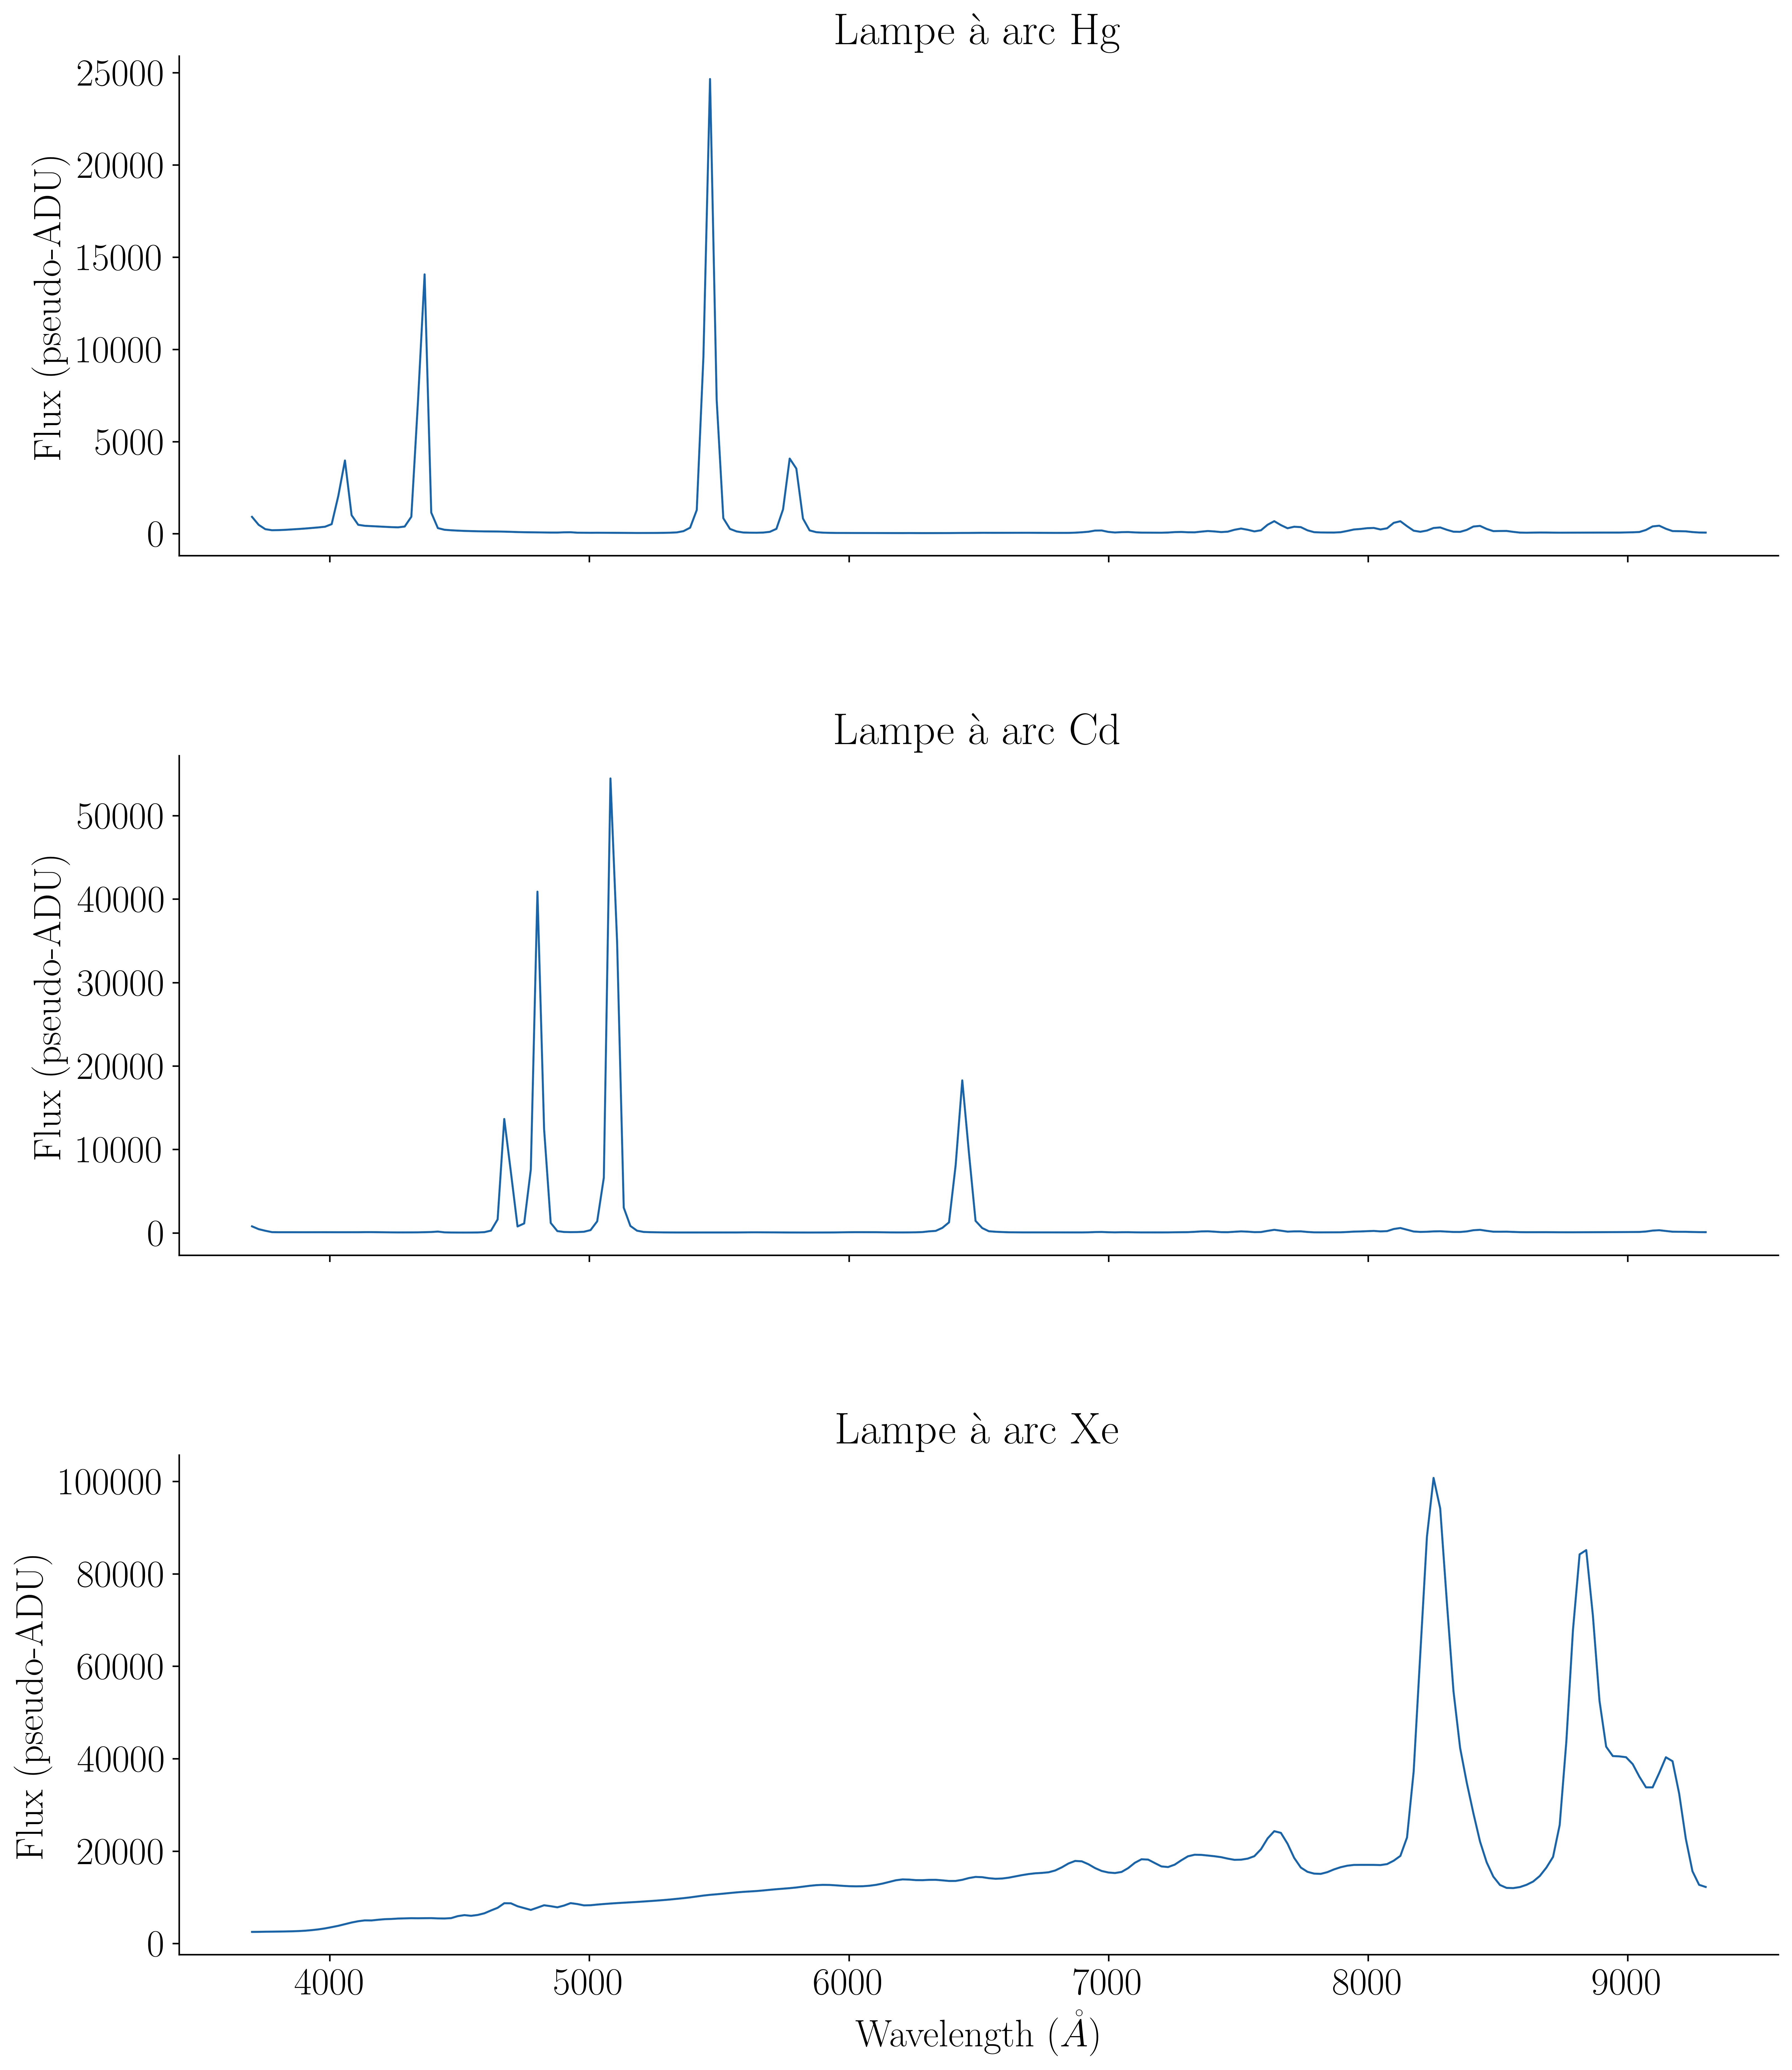
\includegraphics[width=0.9\textwidth]{../figures/06_irf/arclamps.png}
  \caption[Spectres des lampes à arc utilisées pour la SEDm]{Spectres
    des lampes à arc utilisées pour la SEDm pour la nuit du 3 Juillet
    2020. De haut en bas, spectre de la lampe à mercure (Hg), à cadmium
    (Cd) et à Xenon (Xe). Ces spectres sont en unité de flux
    (pseudo-ADU) par longueur d'onde, et sont donc reconstruits à partir
  de la solution en longueur d'onde correspondante. Chaque spectre
  correspond au spectre moyen sur tout le MLA.}
  \label{fig:arclamps}
\end{figure}

\subsection{Détermination de la LSF}
% \label{ssec:xxx}

En toute rigueur, chaque spaxel possède sa propre réponse
impulsionnelle, et il faudrait déterminer la LSF pour chacun d'entre
eux. En pratique, nous faisons la supposition que la LSF moyenne sur
tout le MLA est suffisamment représentative de la réponse impulsionnelle
spectrale de la SEDm à l'échelle locale.

Pour prendre en compte une potentielle variation de la LSF au cours du
temps, nous utilisons les solutions en longueurs d'onde de $65$ nuits
étalées entre 2018 et 2022. Nous récupérons ainsi les positions et
écarts types modélisés pour chaque raie d'émission pour chaque spaxel de
chaque nuit. La solution en longueur d'onde nous permet également de
passer de passer de l'espace des pixels du CCD à l'espace des longeurs d'onde.

Nous utilisons la médiane de la localisation fittée de chaque raie
parmi tous les
spaxels, de même pour les écarts types, afin d'éviter les potentiels
outliers, notamment sur les bords du MLA (voir \citet{pysedm}). Les Figure~\ref{fig:lineloc} et
\ref{fig:linestd} montrent la distribution des localisations et écart
types médians des 65 nuits pour chaque raie d'émission.

On observe dans
la majorité des solutions en longueur d'onde un biais systématique par
rapport à la longueur d'onde de la raie de référence de l'ordre de
$3$\AA\ pour les lampes Cd et Hg . Les deux dernières raies de Xenon sont très peu contraintes, et
on peut apercevoir une dispersion de l'ordre de $20$\AA\ entre les
différentes nuits d'étude. 

La distribution des écarts types propres à chaque raie indique bien une
évolution chromatique, avec une résolution spectrale plus fine dans le
bleu que dans le rouge. La dispersion sur les nuits sélectionnées est de
l'ordre de quelques \AA.

\begin{figure}[h!]
  \centering
  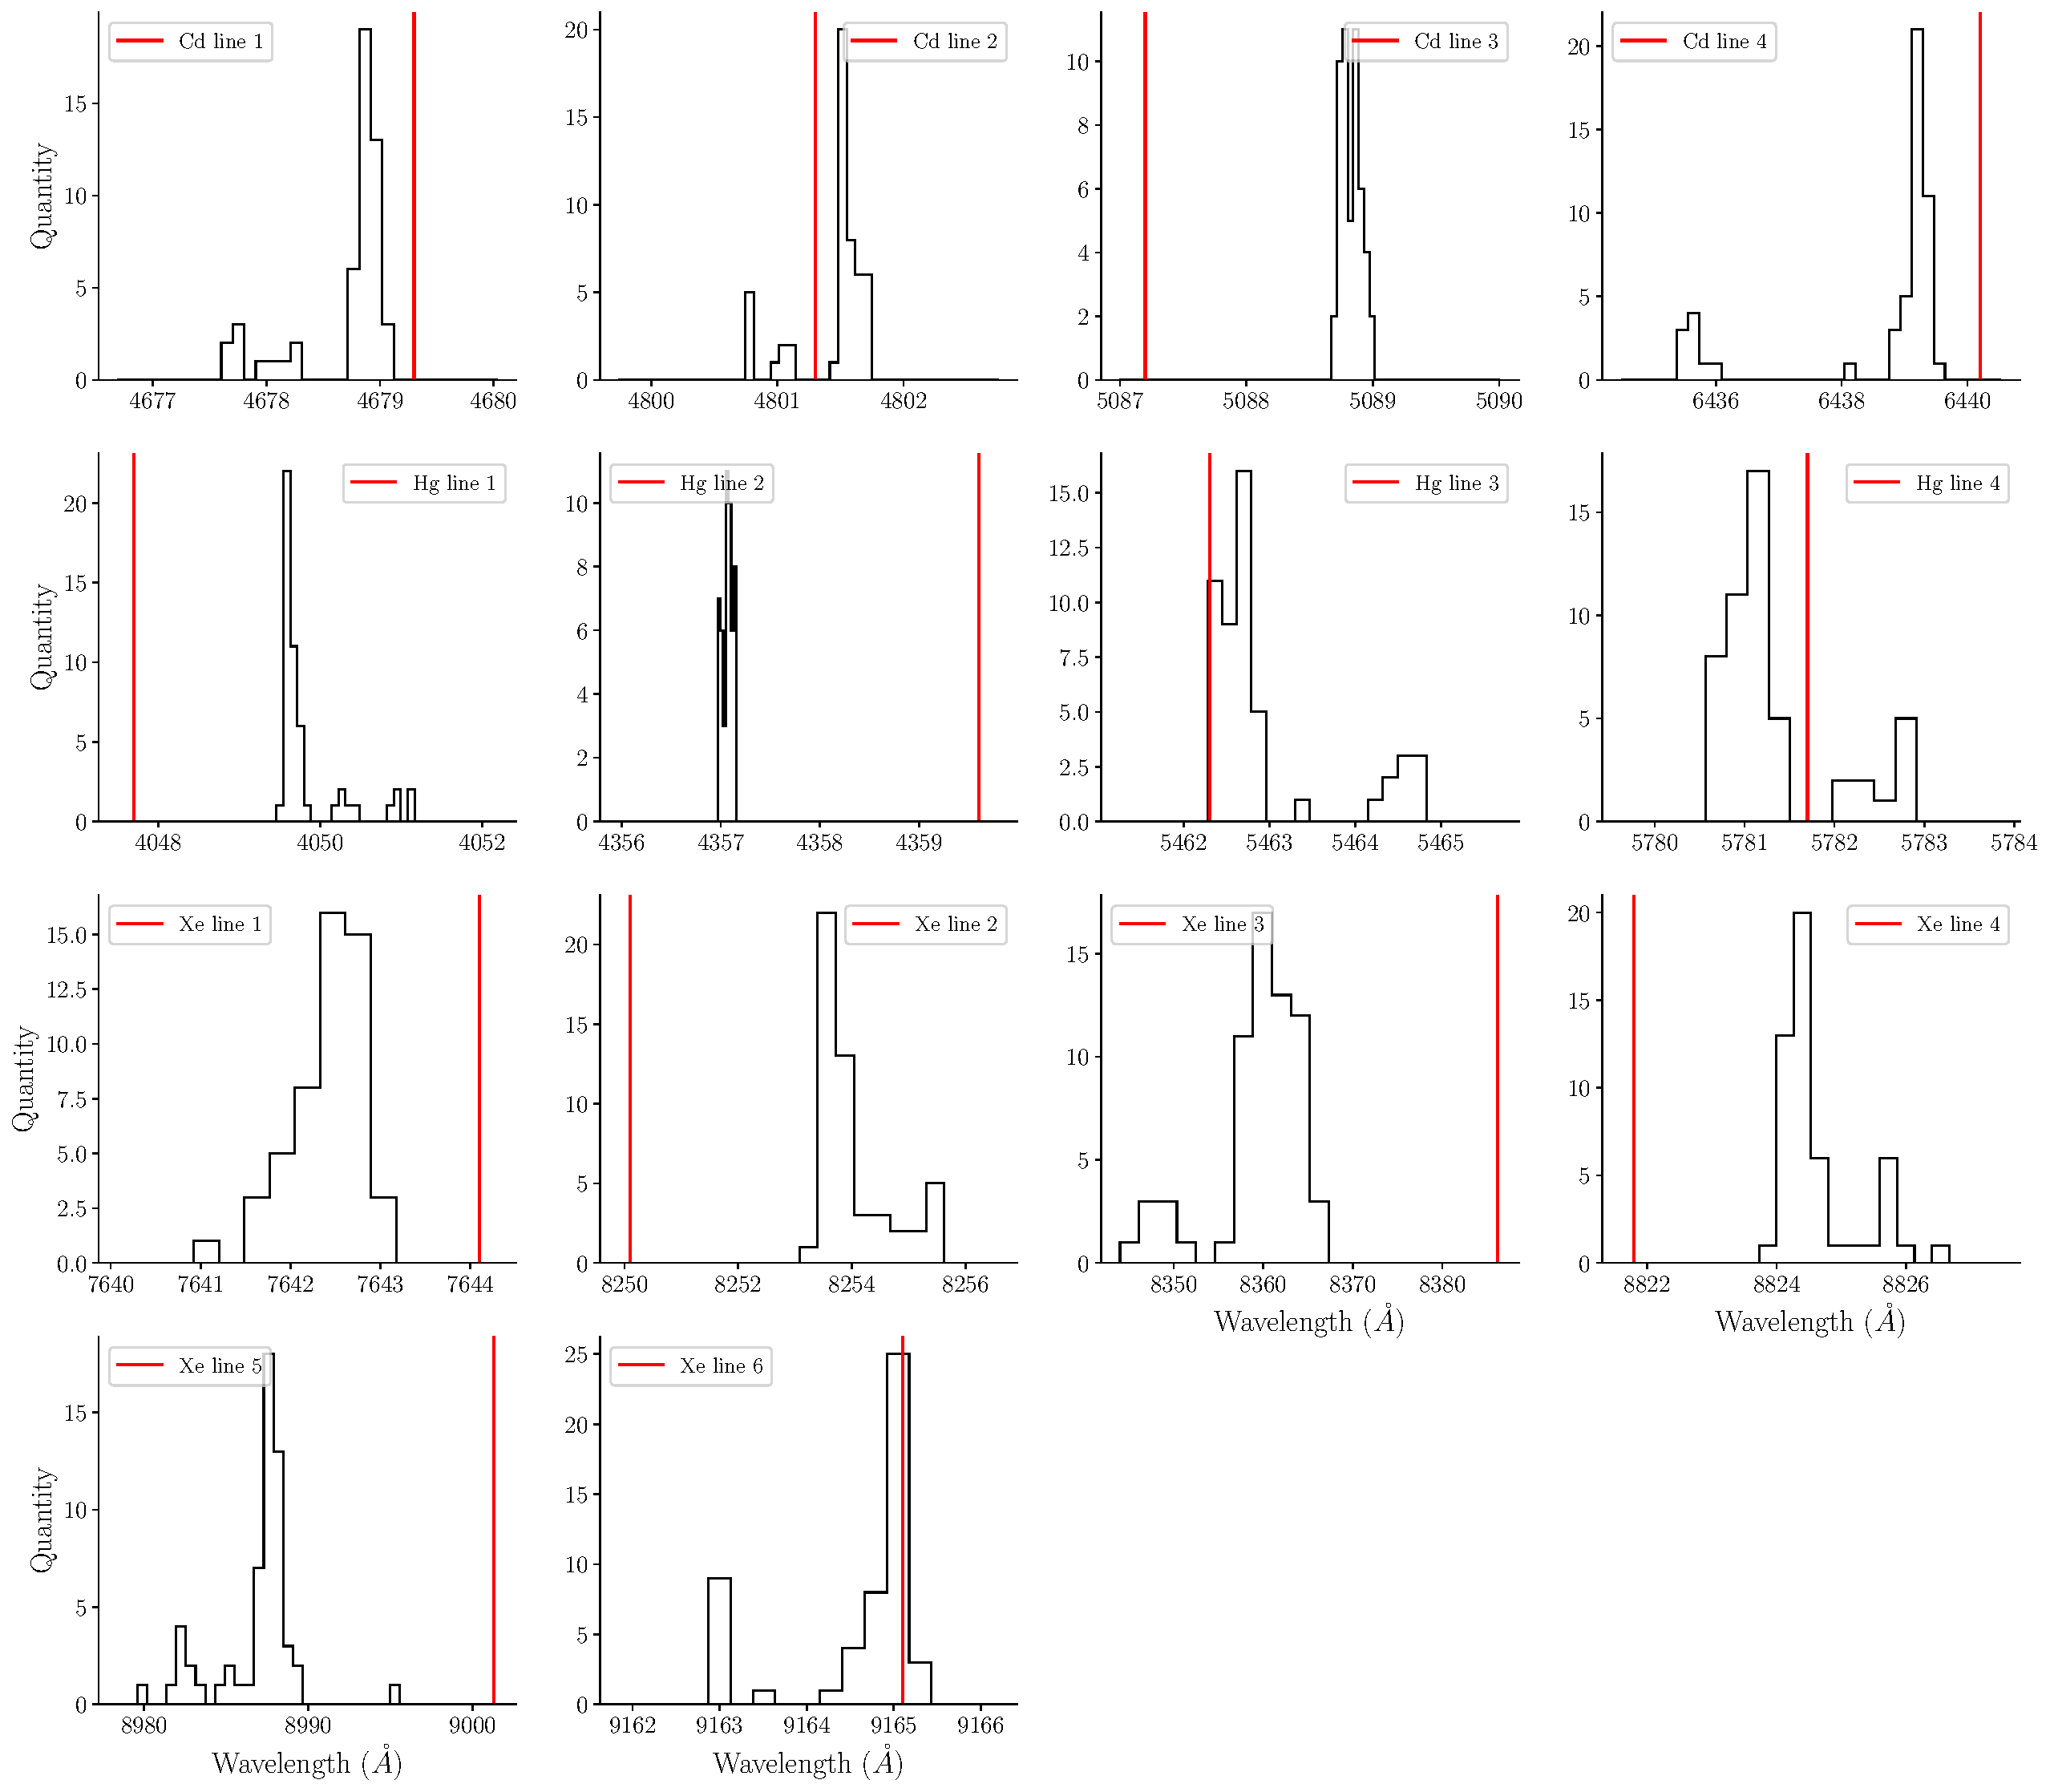
\includegraphics[width=0.99\textwidth]{../figures/06_irf/lineloc.pdf}
  \caption[Distribution de la localisation des raies des lampes à
  arc]{Distribution de la localisation des raies des lampes à arc, en
    considérant la position médiane sur tous les spaxels du MLA pour la
    solution en longueur d'onde de 65 nuits entre 2018 et 2022. La
    localisation rouge verticale indique la position de la raie
    d'émission pour
    chaque lampe suivant les valeurs de la
    Table~\ref{tab:linearclamp}.}
  \label{fig:lineloc}
\end{figure}


\begin{figure}[h!]
  \centering
  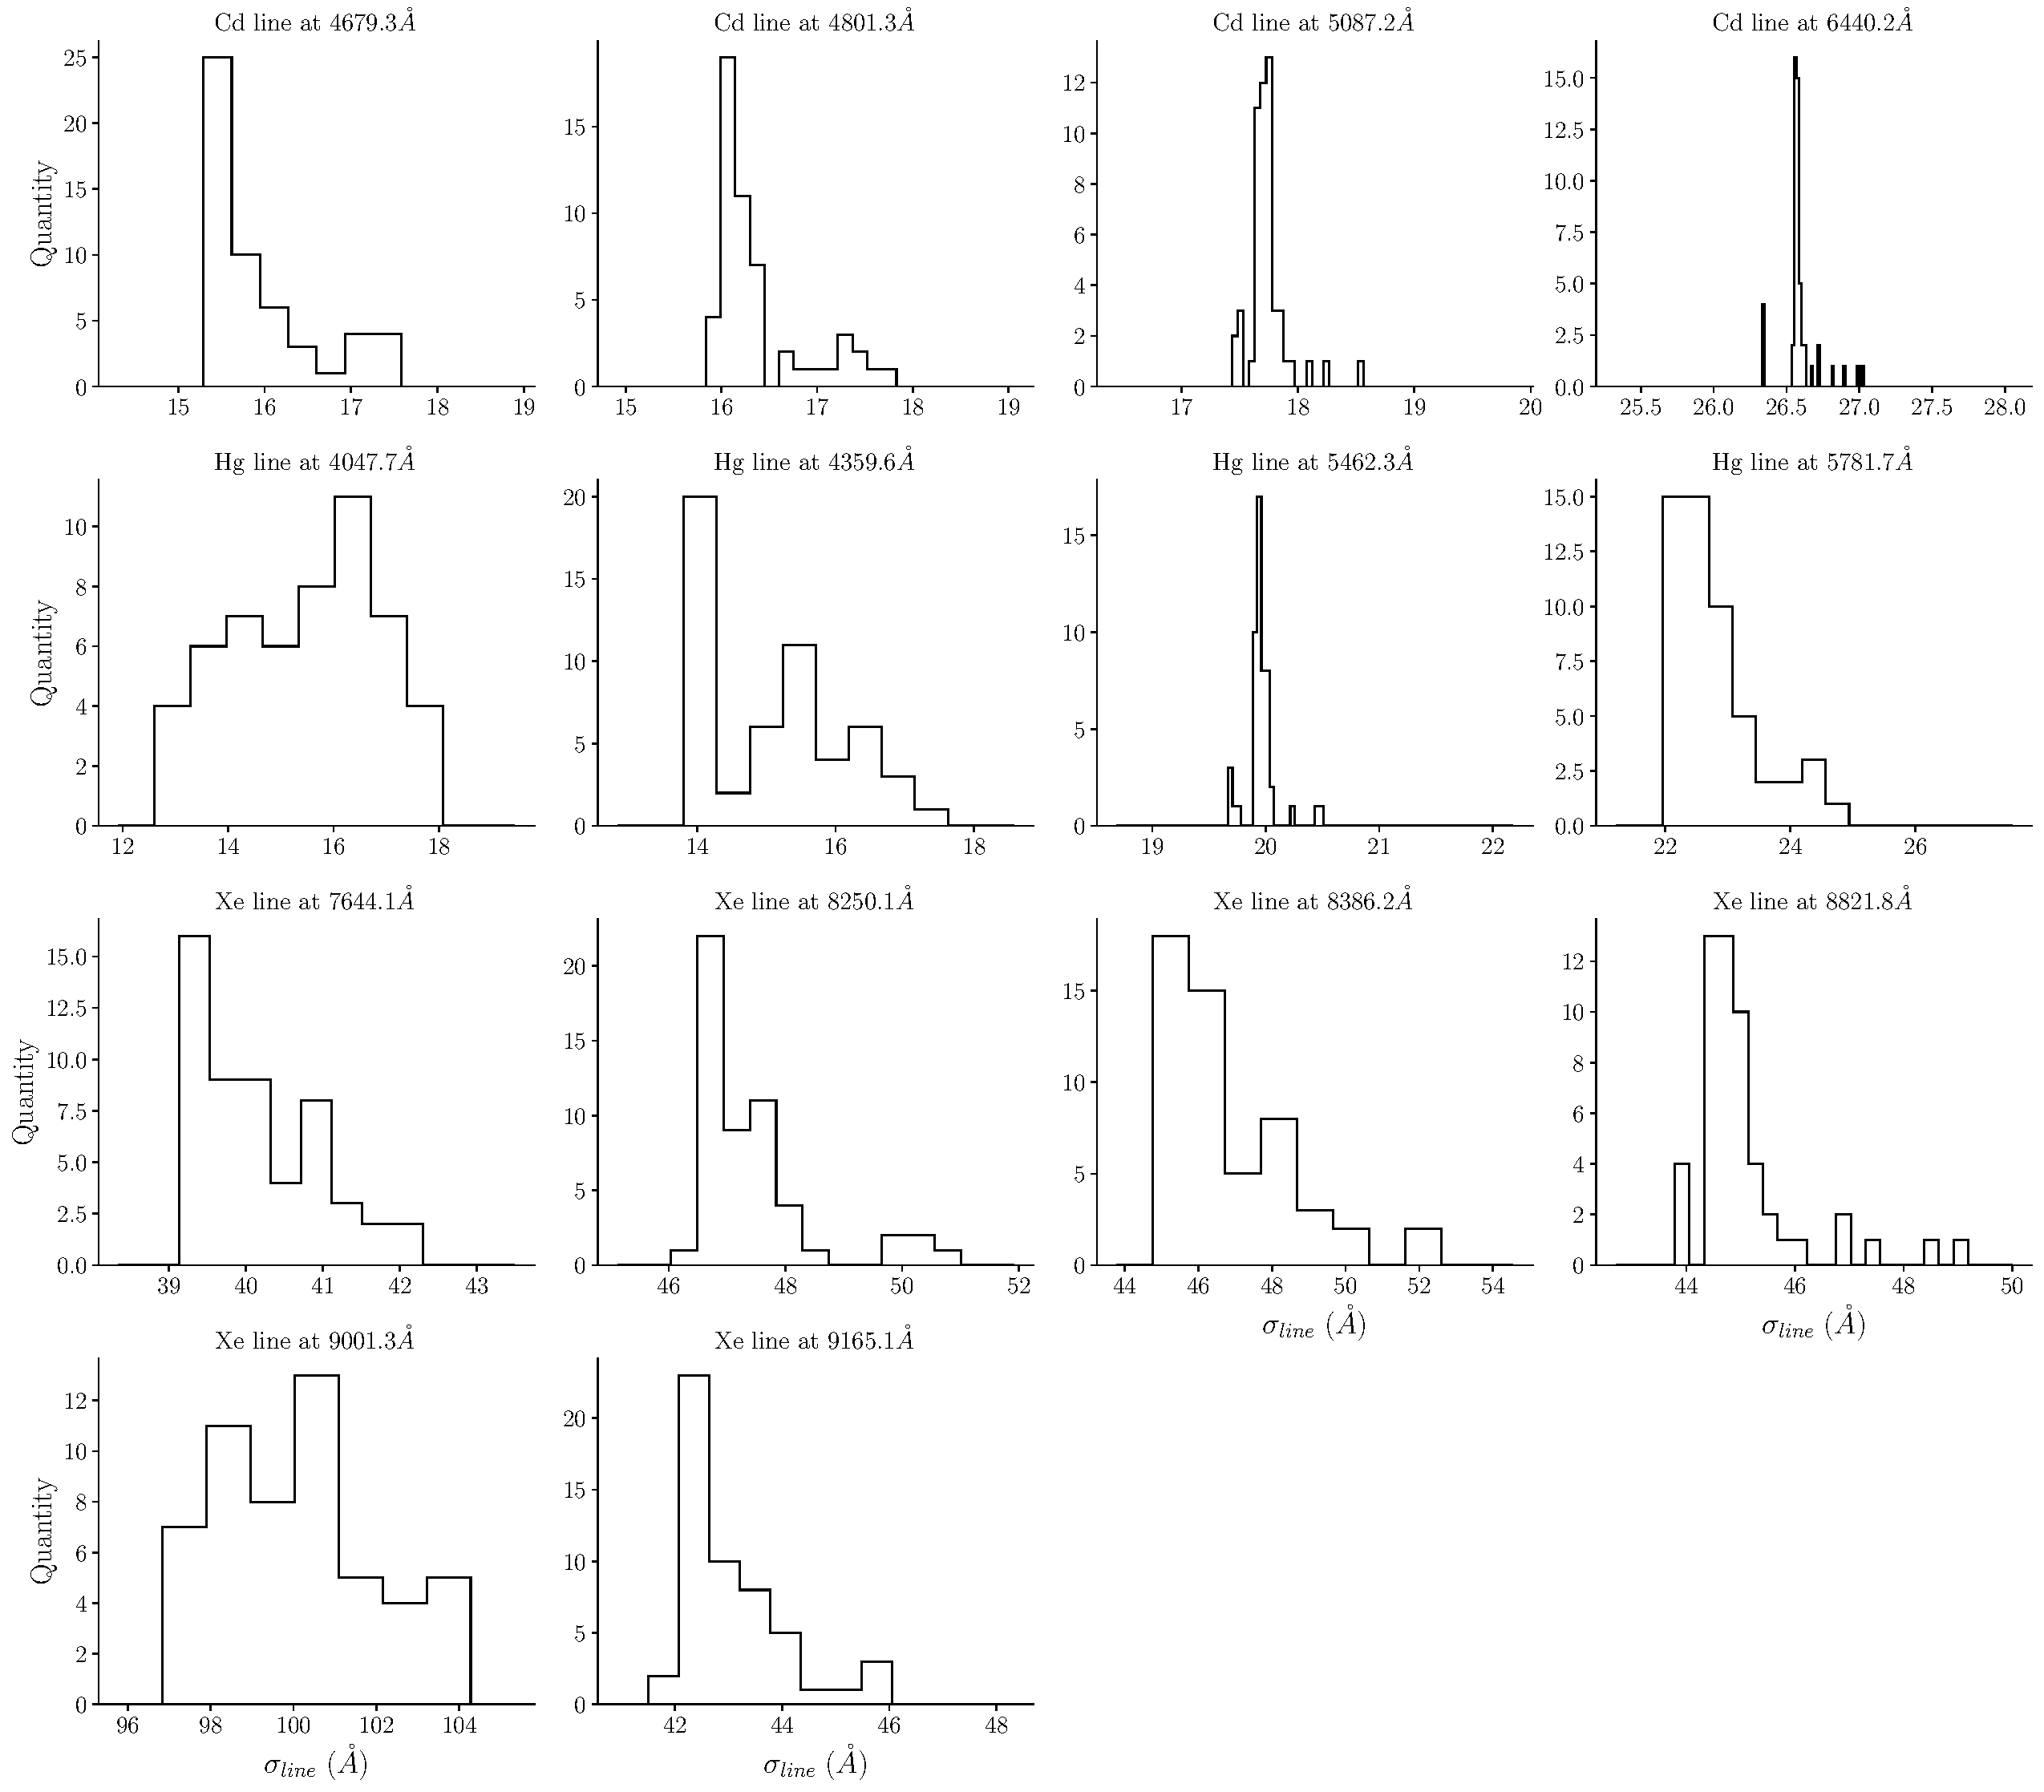
\includegraphics[width=0.99\textwidth]{../figures/06_irf/linestd.pdf}
  \caption[Distribution de l'écart type $\sigma_{line}$ des raies des
  lampes à arc]{Distribution de l'écart type $\sigma_{line}$ des raies
    des lampes à arc, en
    considérant l'écart type médian sur tous les spaxels du MLA pour la
    solution en longueur d'onde de 65 nuits entre 2018 et 2022.}
  \label{fig:linestd}
\end{figure}

Sachant que les raies d'émission de la lampe à Xenon sont faiblement
contraintes, nous choisissons de modéliser la chromaticité de la LSF en
utilisant une combinaison linéaire de polynomes de Legendre de degré 2, afin d'éviter un effet
d'over-fitting aux extrémités.

Pour rappel, les polynômes de Legendre sont
constitués d'une suite de polynômes $p_{n}(x)$ de degré
$n$, et tous les polynômes de la suite sont orthogonaux deux à deux.

On peut les définir sous forme de somme tel que:

\begin{equation}
  \label{eq:legendre}
  P_{n}(x)=\frac{1}{2^{n}}\sum\limits^{n}_{k=0}\binom{n}{k}^{2}(x-1)^{n-k}(x+1)^{k}
\end{equation} 

Notre modèle de LSF chromatique est donc exprimé tel que:
\begin{equation}
  \label{eq:lsfmodel}
  \sigma(\lambda)=\sum\limits_{i}^{n=2}C_{i}P_{i}(\lambda)
\end{equation}

Avec$P_{i}$ étant les polynomes de Legendre de degré $i$ et les $C_{i}$
les coefficients associés. Nous montrons dans la Figure~\ref{fig:lsf} la modélisation de la LSF
chromatique, avec les coefficients $C_{i}$ fittés:

\begin{align*}
  C_{0}&=19.65\pm 0.32\\
  C_{1}&=26.0\pm 0.6\\
  C_{2}&=7.3\pm 0.6
\end{align*}

Pour des raisons de clareté visuelle, nous avons choisi de montrer sur
la Figure~\ref{fig:lsf} la distribution des écarts types sous forme de
violon, la dispersion de la position de la raie étant trop faible pour
être discernable sur la figure. Nous présentons la LSF
$\sigma_{\lambda}$ en unité de longueur d'onde mais également en unité
de tranche équivalente pour la SEDm,
connaissant l'échantillonnage du domaine spectral.

\begin{figure}[h!]
  \centering
  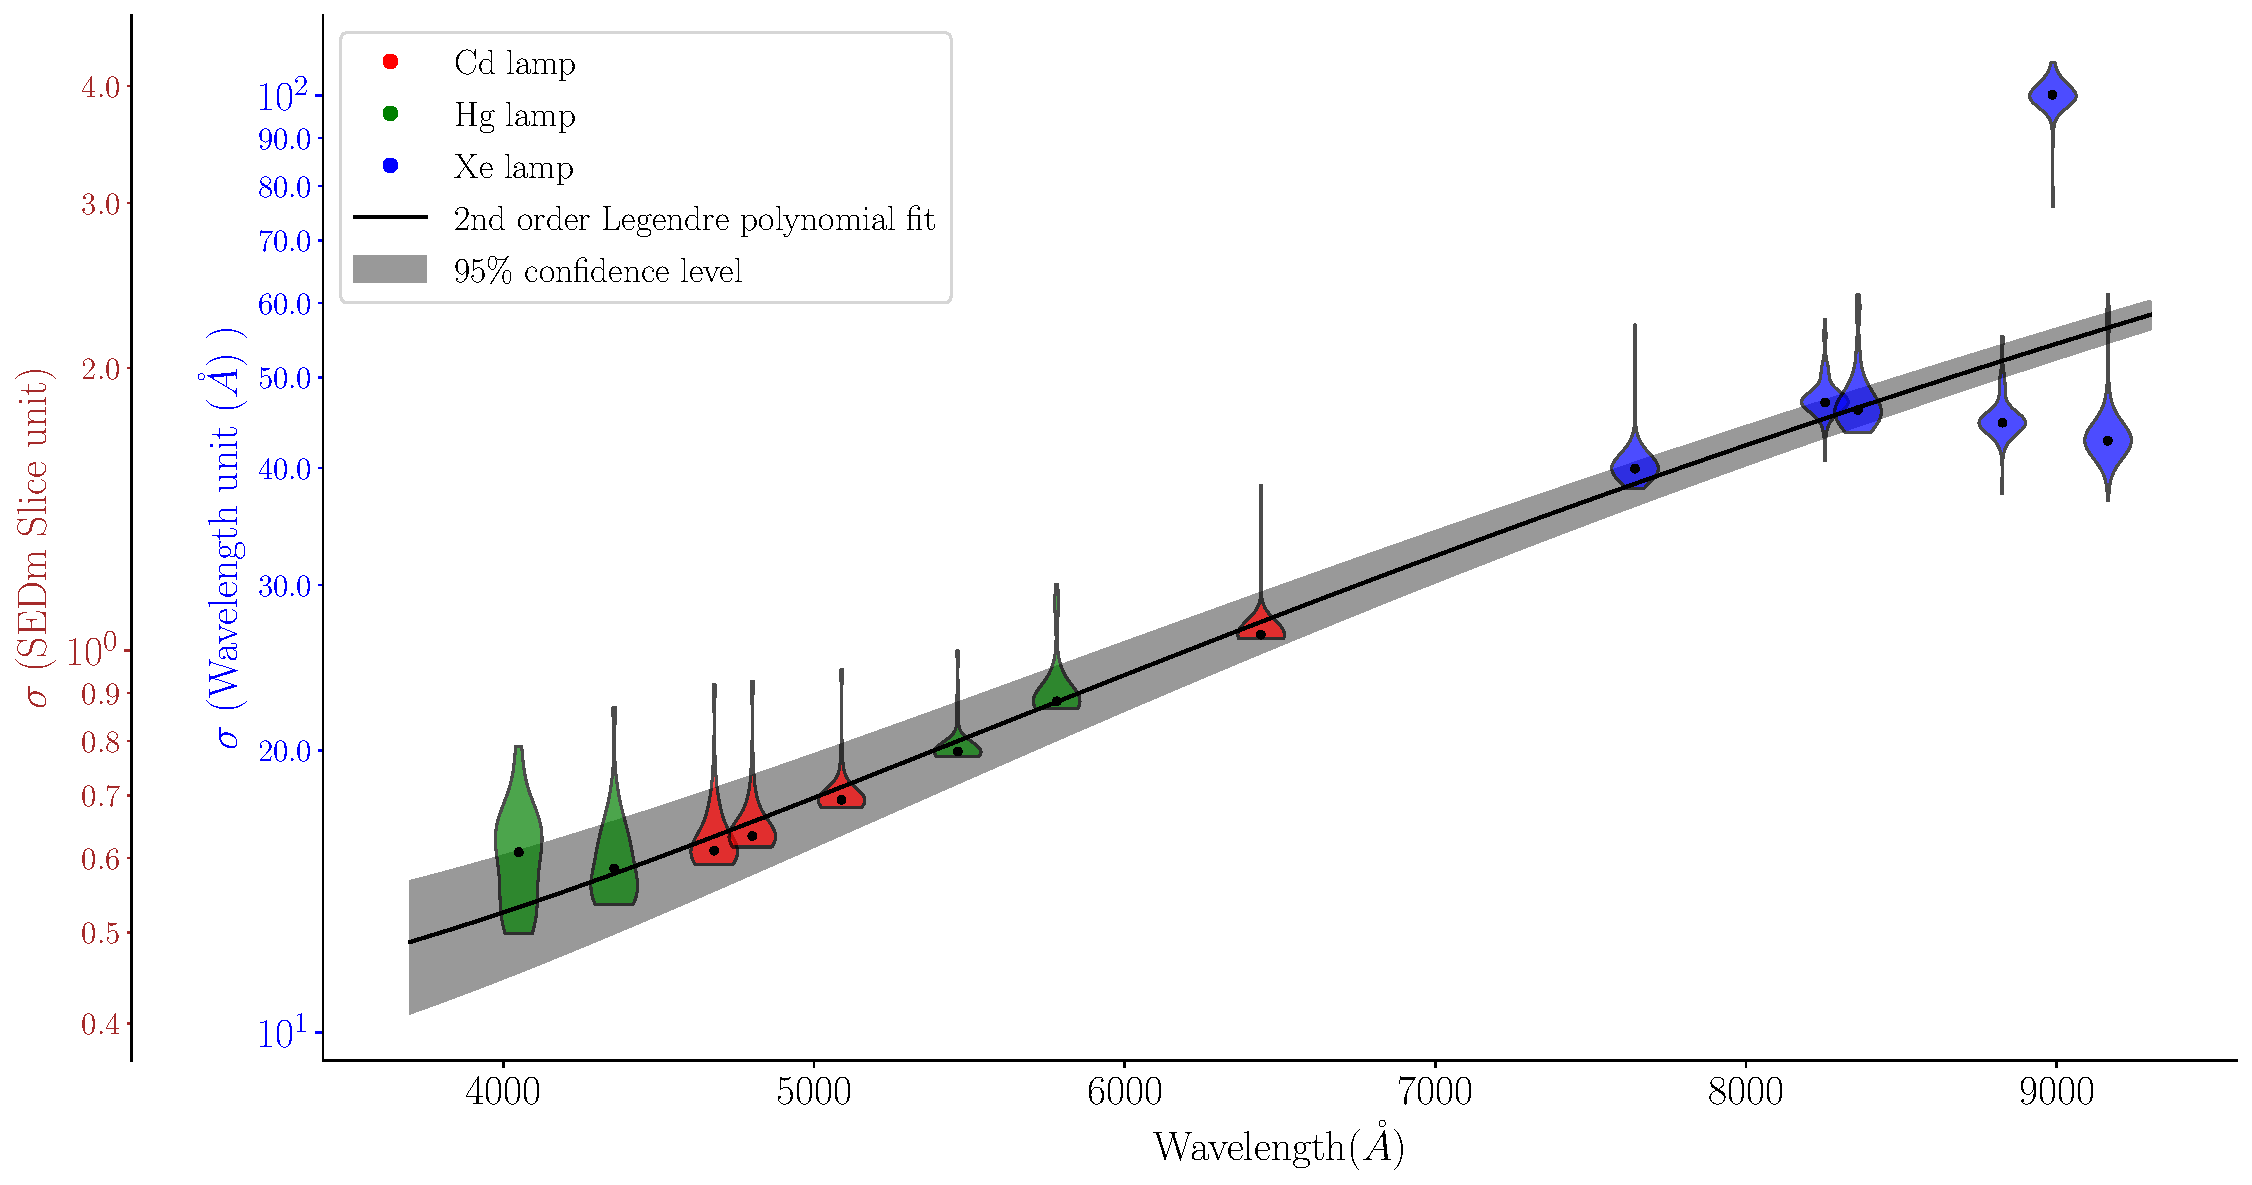
\includegraphics[width=0.99\textwidth]{../figures/06_irf/LSF.pdf}
  \caption[Chromaticité de la LSF]{Chromaticité de la LSF. Nous montrons
  ici l'évolution de l'écart type $\sigma$ des différentes raies
  d'émission pour les lampes à arc Cd, Hg et Xe en fonction de la
  longueur d'onde. L'écart type $\sigma$ est présenté en unité de
  longueur d'onde ($\lambda$[\AA]) et en unité d'épaisseur de tranche
  dans les cubes 3D de la SEDm. Cette étude est réalisée à partir des
  solutions en longueurs d'onde de 65 nuits étalées entre 2018 et
  2022. La dispersion de la position des raies étant très faible et ne
  pouvant par conséquent être discernable sur la figure, nous présentons
la dispersion des $\sigma$ sous forme de violon. Le code couleur indique
la lampe à arc dont est issue la raie d'émission. Le modèle fitté
(polynomes de Legendre d'ordre 2) est présenté en courbe noir, et les
bandes grises indiquent l'erreur du modèle à 2 sigmas. }
  \label{fig:lsf}
\end{figure}

Sachant que la largeur à mi-hauteur (FWHM) pour une distribution
gaussienne est de $\text{FWHM}=2\sqrt{2\ln(2)}\sigma\approx2.355\sigma$, nous
pouvons également caractériser le pouvoir de résolution de la SEDm, que
nous illustrons dans la Figure~\ref{fig:resolutionsedm}.
Comme introduit dans \citet{SEDM18}, la résolution spectrale
$R=\frac{\lambda}{\Delta\lambda}$ est de l'ordre de $100$ sur tout le
domaine spectral. Néanmoins, nous pouvons apercevoir que cette
résolution spectrale décroît vers le rouge, avec
$R_{\lambda=4000\mathring{A}}\sim135$,
$R_{\lambda=6500\mathring{A}}\sim100$ et $R_{\lambda=8500\mathring{A}}\sim80$.\\

\begin{figure}[h!]
  \centering
  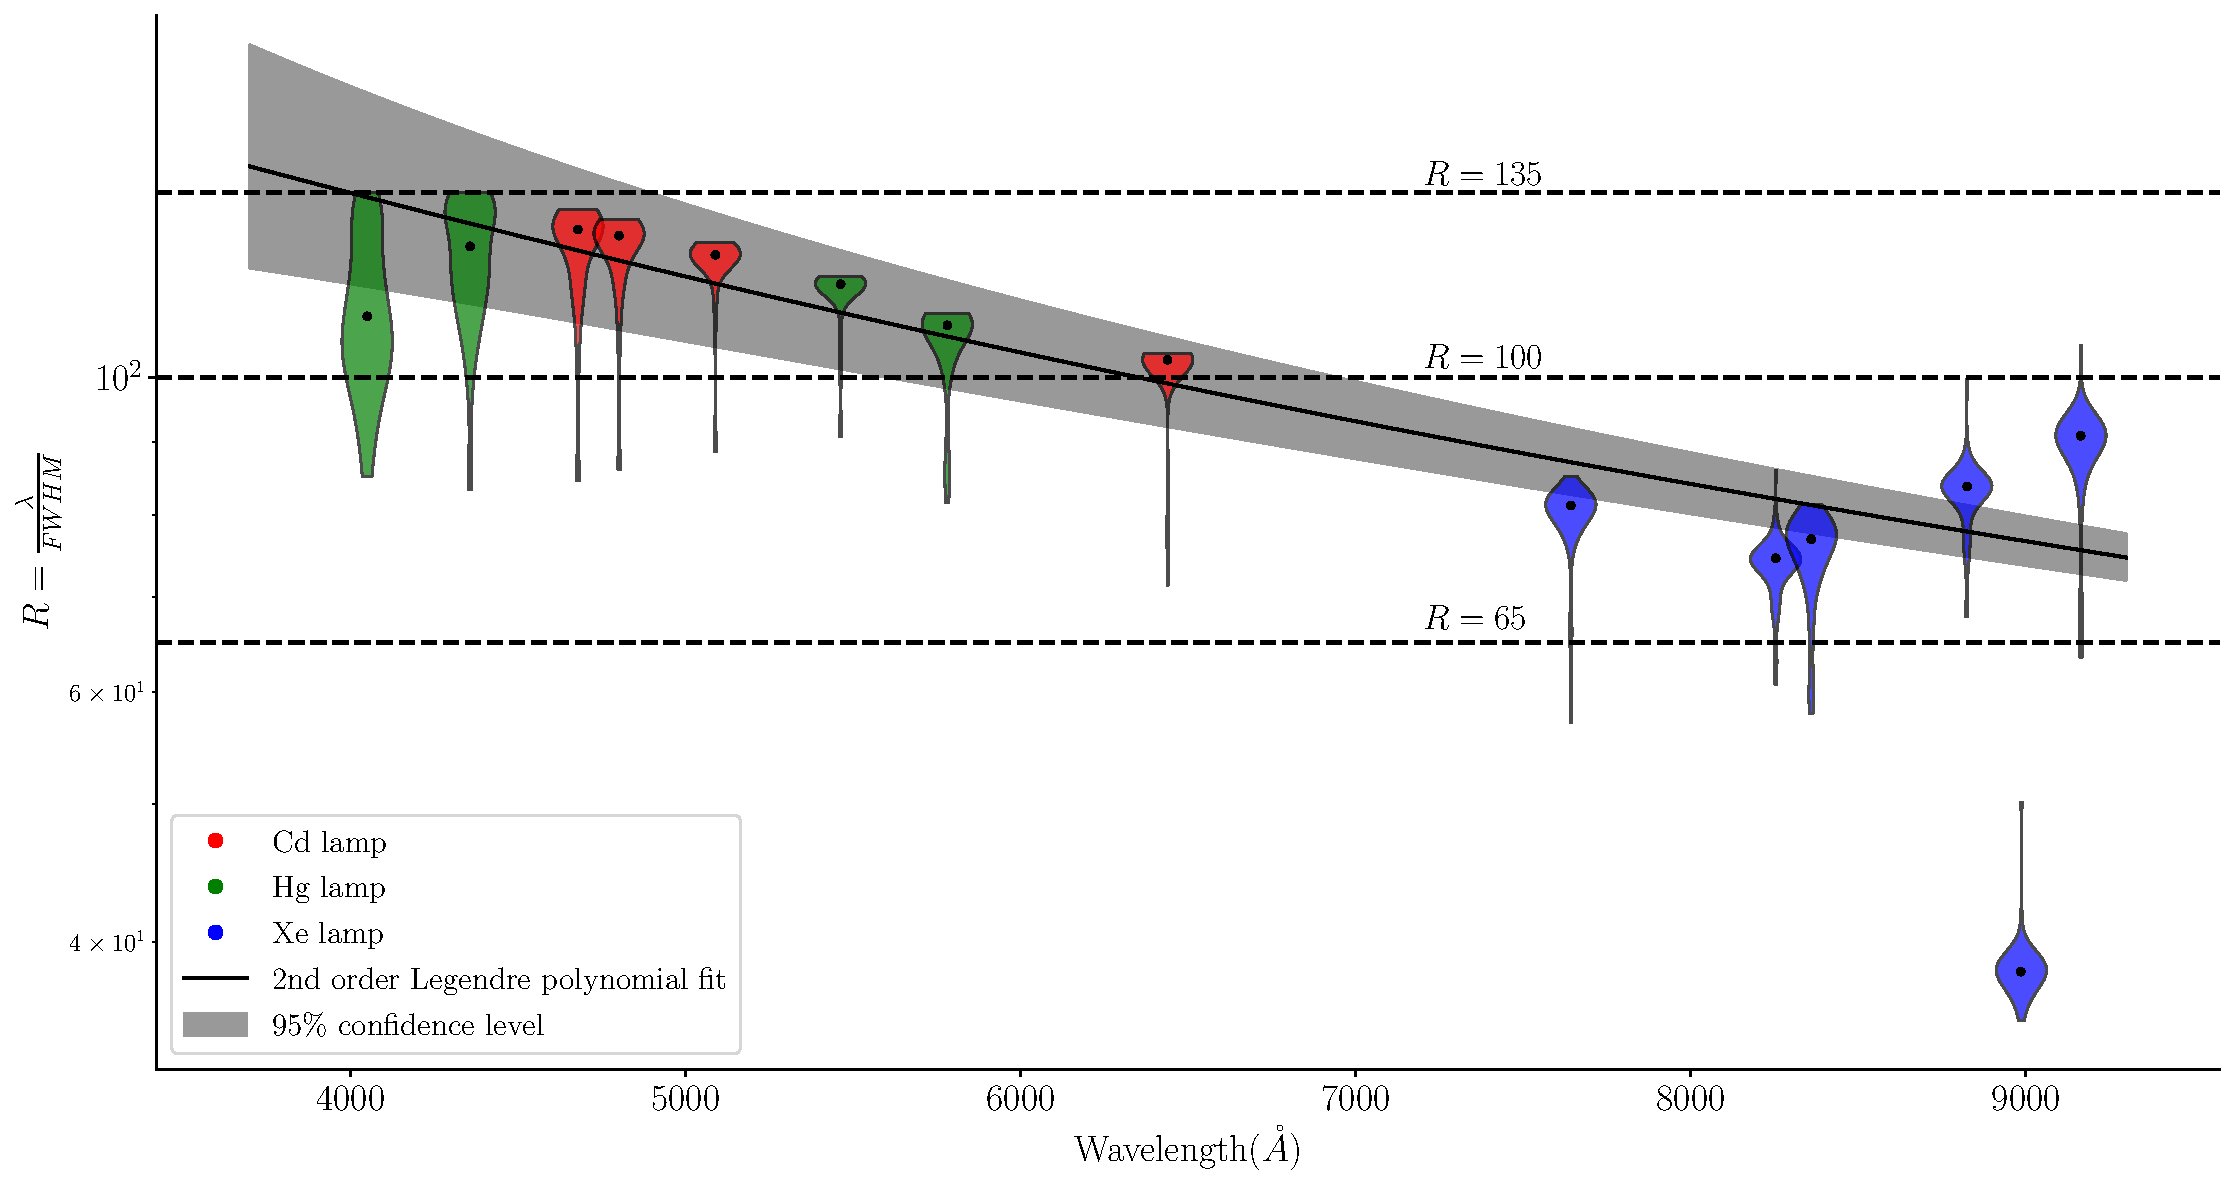
\includegraphics[width=0.99\textwidth]{../figures/06_irf/SEDmResolution_wmodel.pdf}
  \caption[Résolution de la SEDm]{Résolution de la SEDm, où
    $R=\frac{\lambda}{\Delta\lambda}$, avec $\lambda$ la longueur d'onde
  de la raie d'émission et $\Delta\lambda$ leur largeur à mi
  hauteur. Un violon correspond à la distribution en résolution à la
  position d'une raie d'émission (code couleur pour l'origine de la
  lampe) dans le même esprit que dans la Figure~\ref{fig:lsf}. Les lignes horizontales en pointillées indiquent les
  résolutions $R=135$, $100$ et $65$. La description de la SEDm
  \citep{SEDM18} indique une résolution $R\sim100$, ce qui est l'ordre
  de grandeur que nous retrouvons ici.}
  \label{fig:resolutionsedm}
\end{figure}


%\begin{figure}
%\centering
%\begin{subfigure}[b]{0.99\textwidth}
%  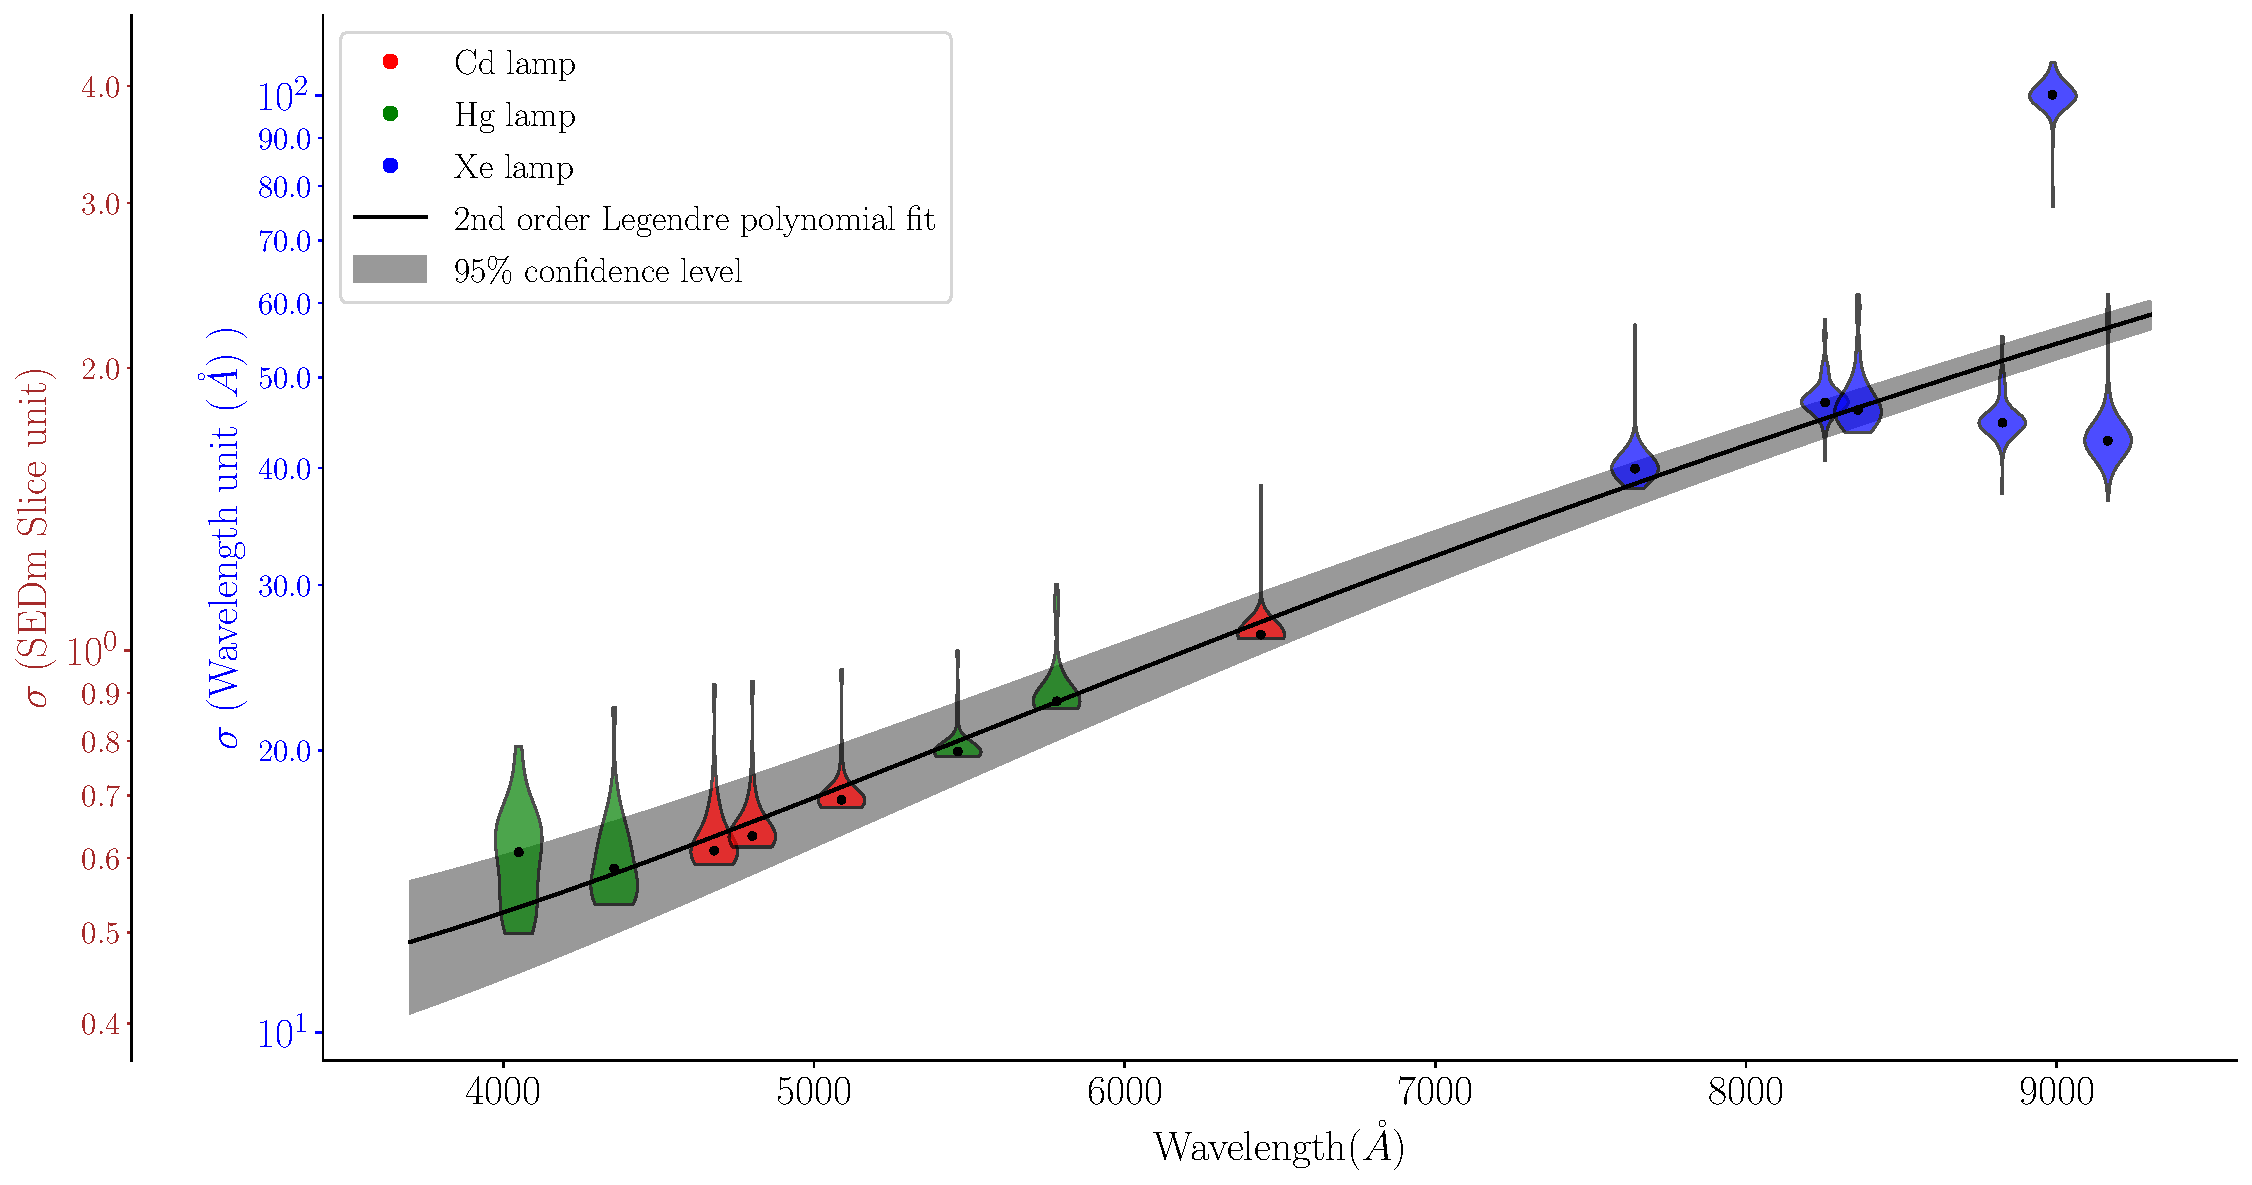
\includegraphics[width=1\linewidth]{../figures/06_irf/LSF.pdf}
%   \caption{Chomaticité de la réponse impulsionnelle spectrale (LSF) de
%     la SEDm}
%   \label{fig:Ng1} 
%\end{subfigure}

%\begin{subfigure}[b]{0.99\textwidth}
%   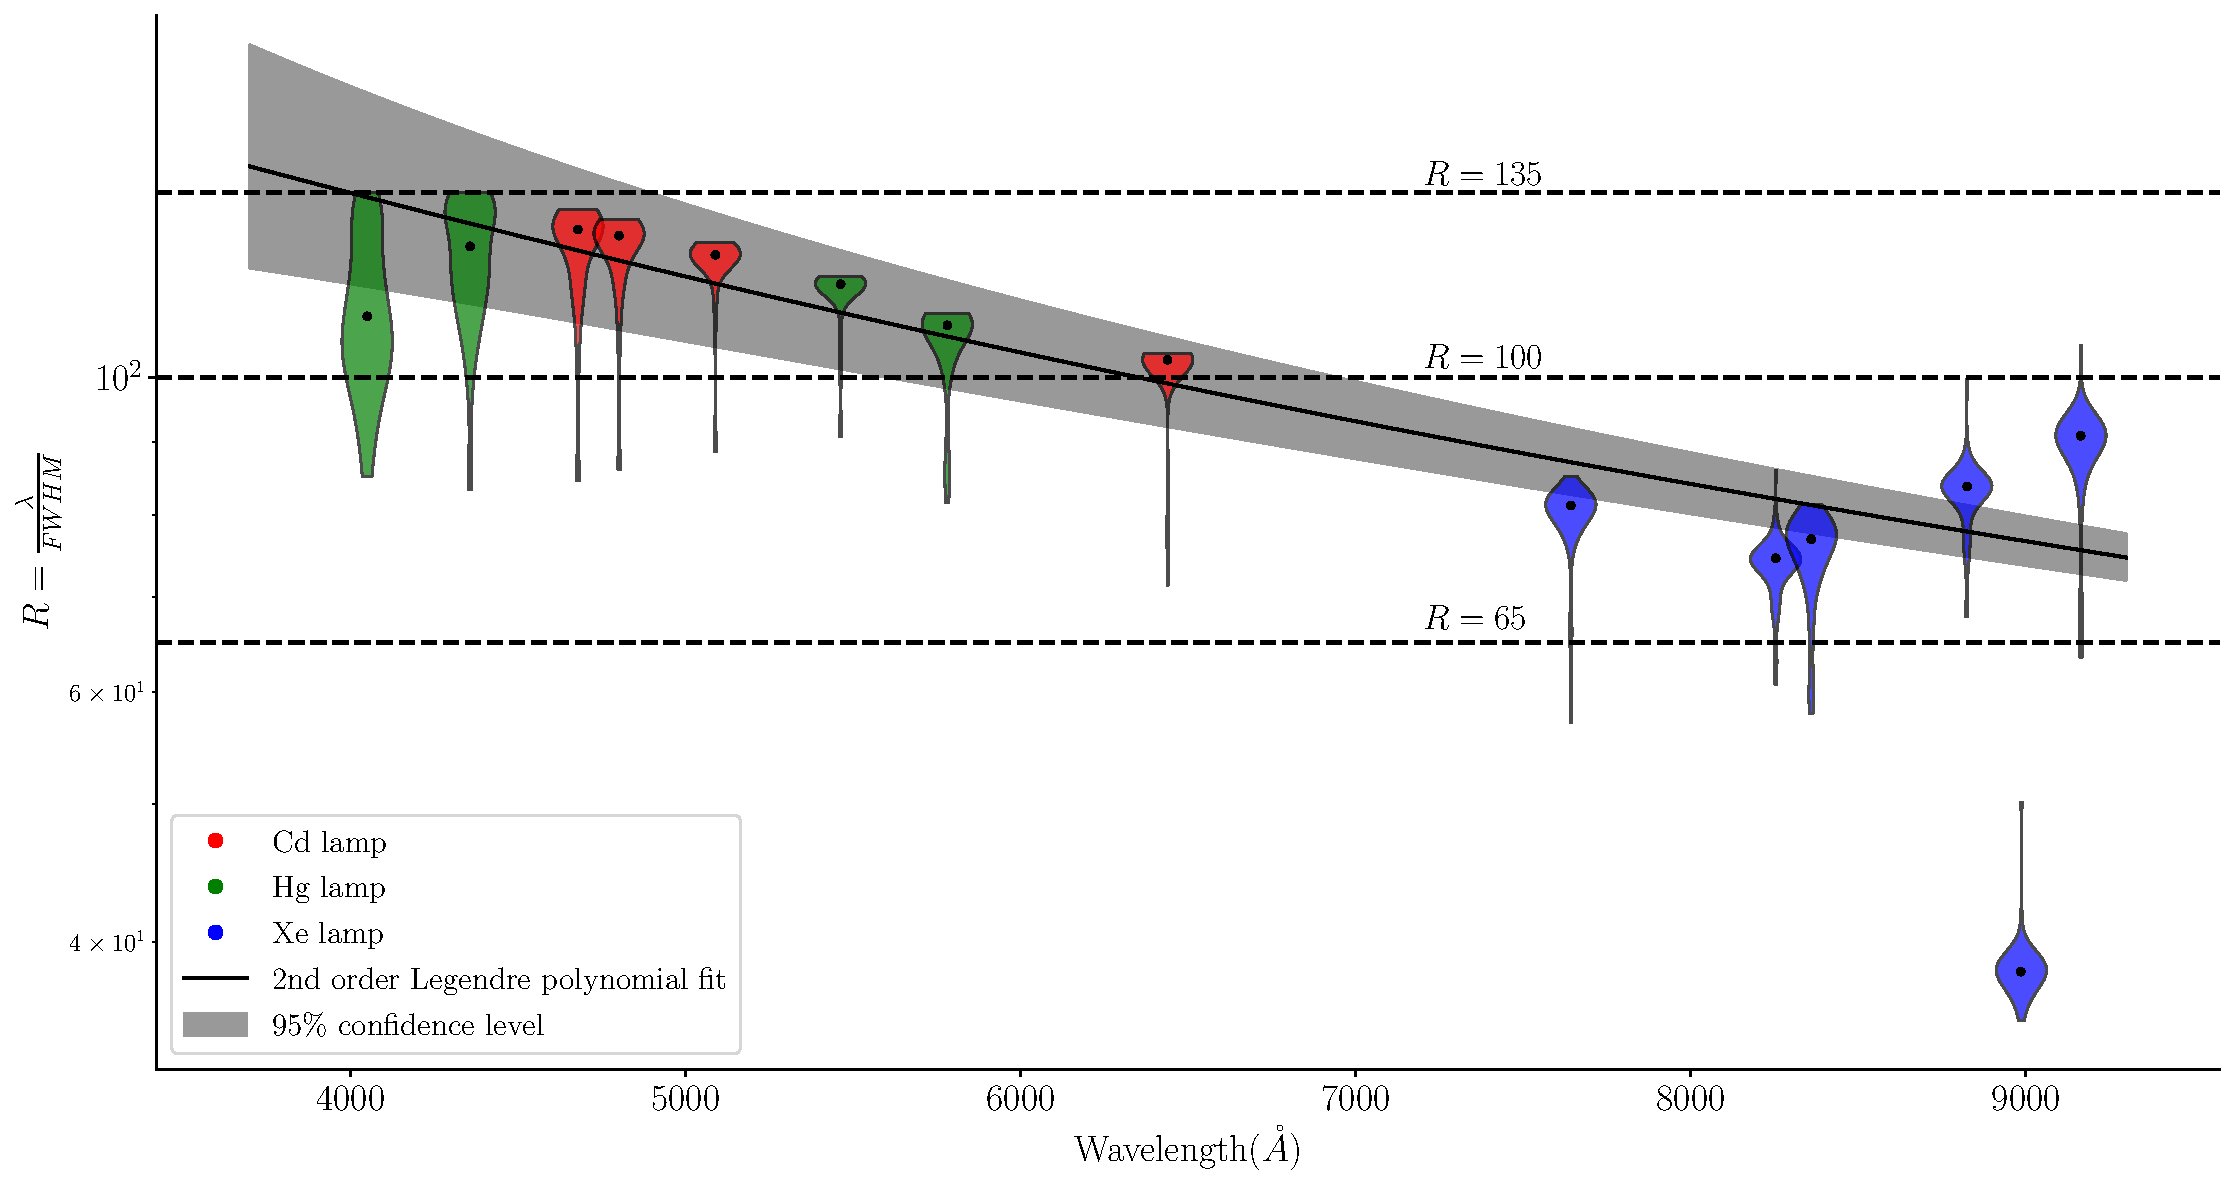
\includegraphics[width=1\linewidth]{../figures/06_irf/SEDmResolution_wmodel.pdf}
%   \caption{Résolution de la SEDm}
%   \label{fig:Ng2}
% \end{subfigure}
%\caption[blavla]{blablabla}
%\end{figure}

Nous fixons ainsi le modèle chromatique de LSF de la SEDm. Sachant que la résolution
des spectres obtenus avec \cigale est de l'ordre de $3$\AA\ sur
l'intervalle [$3200$-$9500$]\AA\ (correspondant à une résolution de
$R=\lambda/\d\lambda\approx2000$; \citet{BCO3}), nous choisissons
de convoluer directement les spectres du cube intrinsèque par la LSF de
la SEDm.

Cette convolution a donc la particularité d'être effectuée avec un
kernel gaussien ayant un écart type variable. Pour effecter
numériquement cette
transformation, nous procédons à un
étirement des spectres par l'inverse de la largeur du kernel à une
position donnée. Nous pouvons alors effectuer une convolution avec un
kernel fixe, puis ``reformer'' les spectres à leur échelle initiale.

La Figure~\ref{fig:lsfapplied} montre par exemple l'application du
modèle de LSF sur le spectre d'un spaxel du cube intrinsèque (le spectre
rouge de la Figure~\ref{fig:cigalesampling} après
ré-échantillonnage). Le lissage progressif et croissant avec la
longueur d'onde dû à la chromaticité de la LSF est
clairement visible.

\begin{figure}[h!]
  \centering
  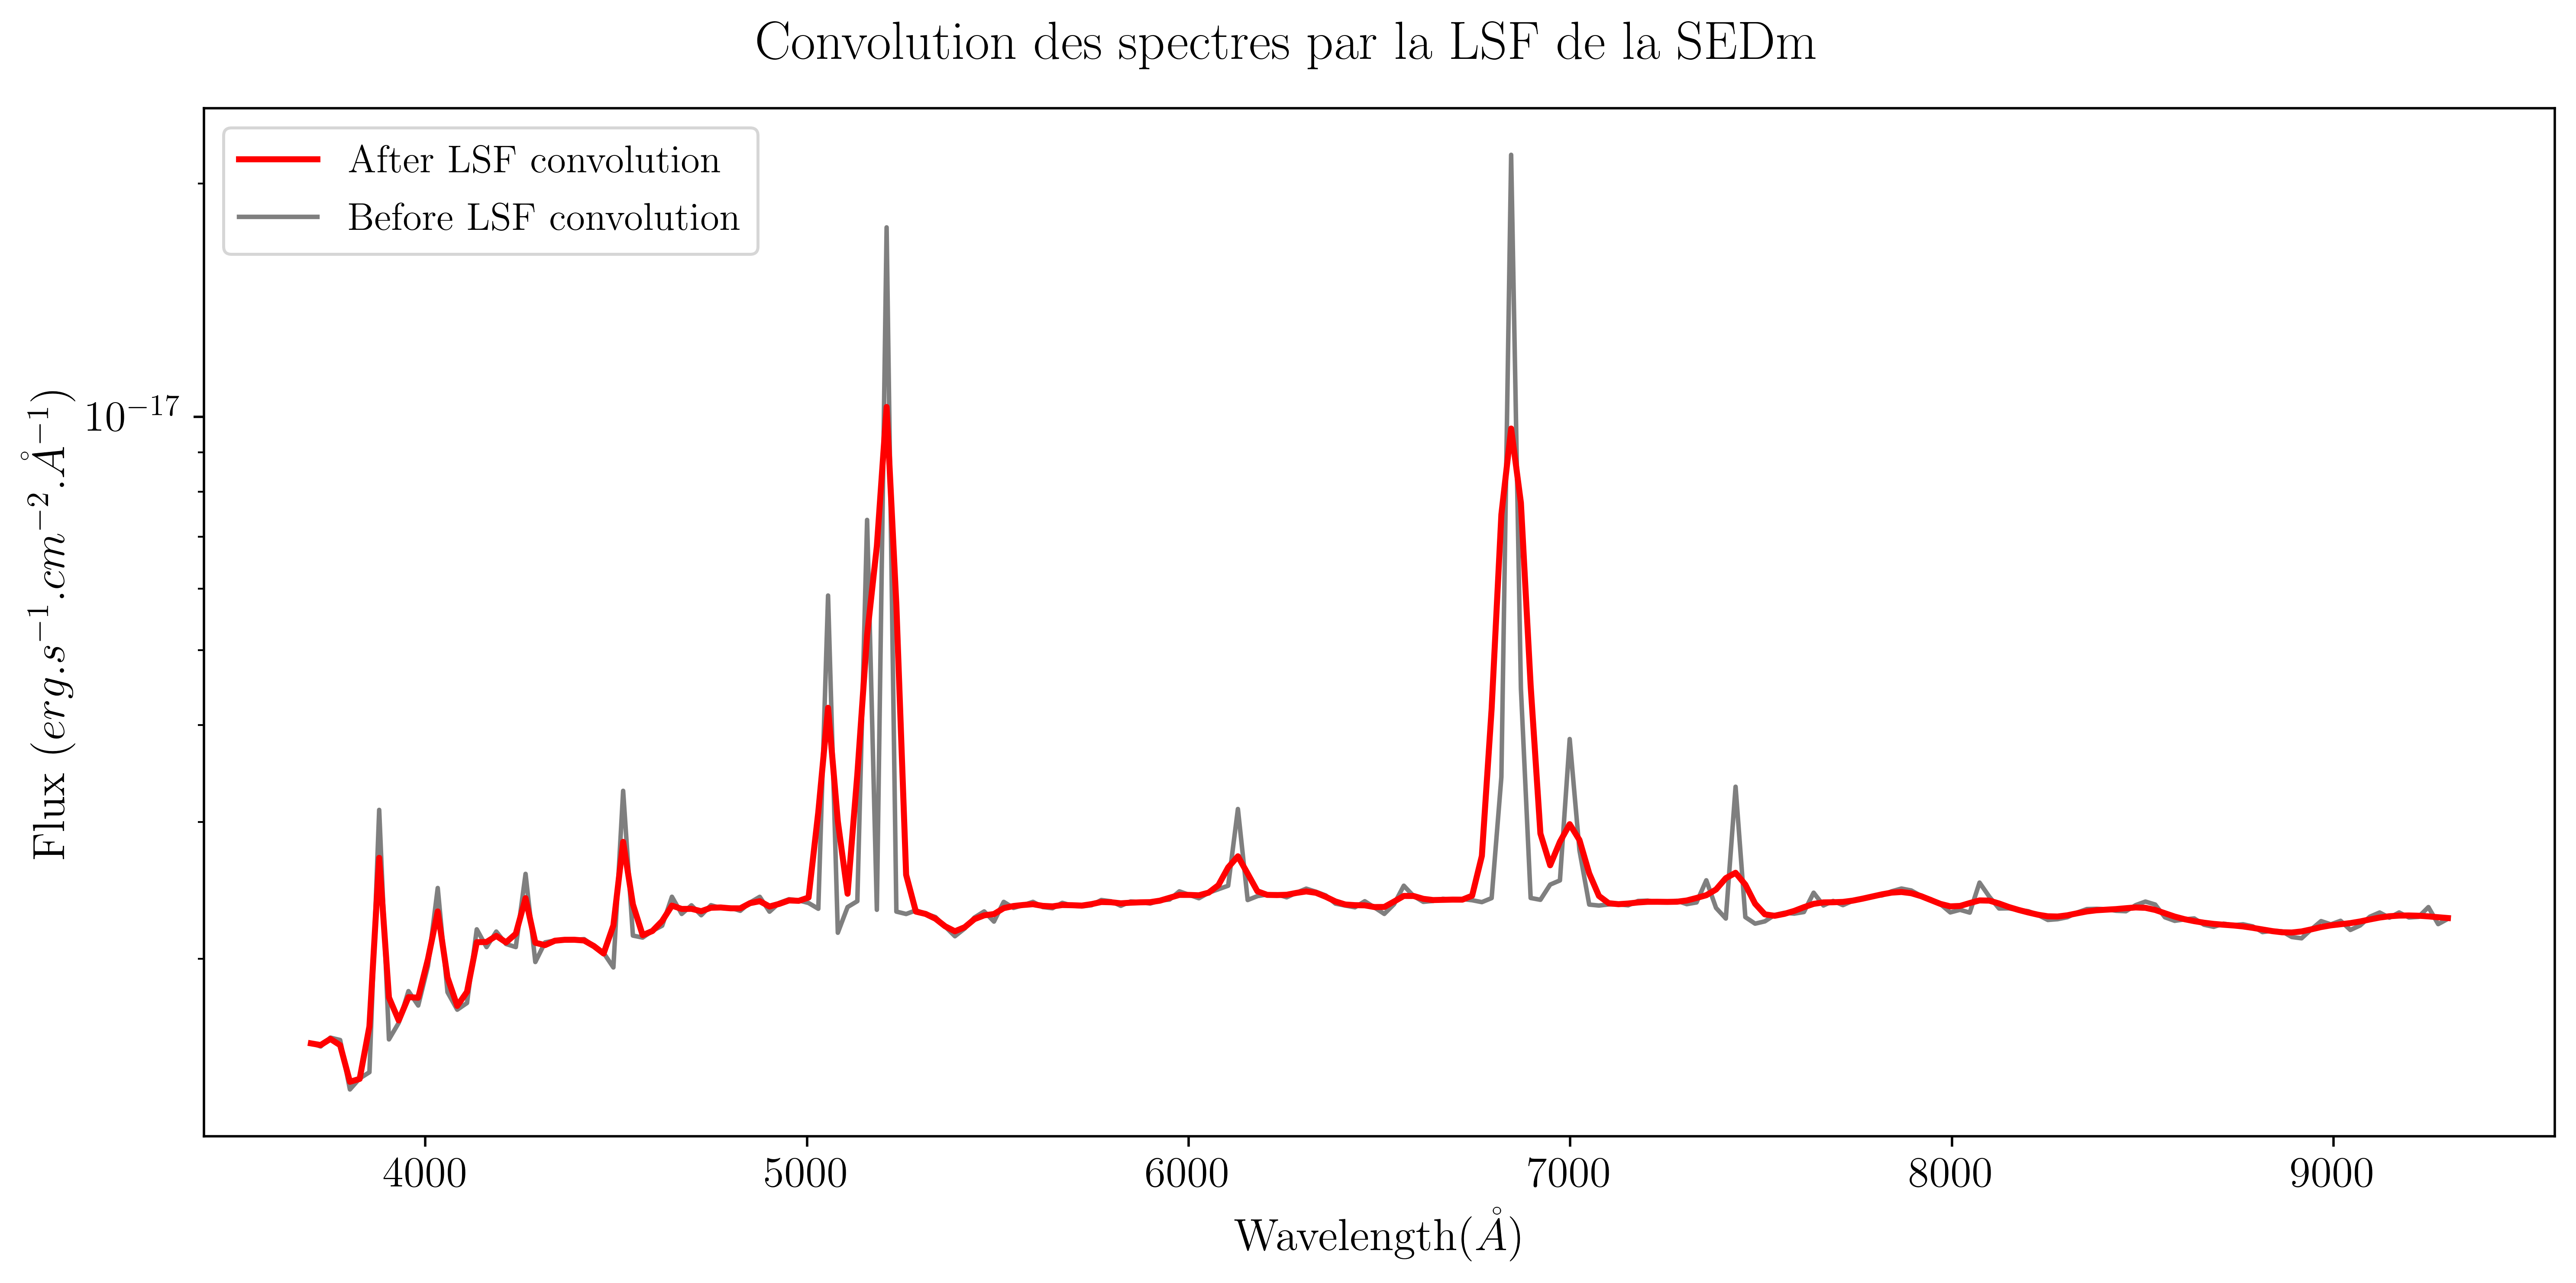
\includegraphics[width=0.99\textwidth]{../figures/06_irf/lsfapplied.png}
  \caption[Application de la LSF]{Application de la LSF aux spectres du
    cube intrinsèque obtenu dans le Chapitre~\ref{sec:intcube}
    (Figure~\ref{fig:intcube_ZTF18accrorf}). Nous montrons ici un exemple
    de la convolution sur le spectre après ré-échantillonnage de la
    Figure~\ref{fig:cigalesampling} (ici en \textit{noir}). Le lissage progressif et croissant avec la
longueur d'onde dû à la chromaticité de la LSF est
clairement visible. Le résultat de la convolution par le kernel variable
est représenté par le spectre \textit{rouge}.}
  \label{fig:lsfapplied}
\end{figure}

Nous appliquons cette convolution pour tous les spaxels du cube
intrinsèque, ce qui nous permet d'avoir notre galaxie hôte dans l'espace
spectral de la SEDm.
\clearpage

\section{Réponse impulsionnelle spatiale: PSF}\label{sec:psf}

La section précédente fut consacrée à la caractérisation de la réponse
impulsionnelle spectrale de la SEDm. Nous présentons ici celle de la
réponse impulsionnelle spatiale, faite à partir d'observations d'étoiles standards (STDs) qui
sont des sources ponctuelles dans le champ de vue de l'IFS.

En associant l'imperfecion du système optique et la présence des
turbulences atmosphériques \citep{Kolmogorov} dont l'hétérogénéité est dynamique, la structure d'une image
varie aléatoirement au cours du temps dans le champ de vue du
télescope. Une exposition de quelques secondes est habituellement
suffisant pour moyenner ces fluctuations et fixer l'image. Nous
pouvons alors relier  $O(\alpha,\lambda)$ le flux d'une source dans un direction $\alpha$ du
ciel à la longueur d'onde $\lambda$, et $\langle
I(\alpha,\lambda)\rangle$ la moyenne temporelle du flux observé
décrivant l'image obtenue dans le plan focal par la
transformation:

\begin{equation}
  \label{eq:transfertpsf}
  \langle I(\alpha,\lambda)\rangle = O(\alpha,\lambda) \otimes \langle
  S(\alpha, \lambda)\rangle
\end{equation}

Avec $\langle S(\alpha, \lambda)\rangle$ l'image moyenne dans le plan focal d'une
source ponctuelle observée à l'infini, qui n'est autre que notre
fonction d'étalement de point (PSF). Sa transformée de Fourrier, notée
$\langle \widetilde{S}(\alpha, \lambda)\rangle$, est la fonction
de transfert du système optique dans son ensemble, qui n'est autre que
le produit entre la fonction de transfert du télescope achromatique
$T(f)$, et la fonction de transfert de l'atmosphère $B(\lambda, f)$.\\

La caractérisation de la PSF est donc cruciale pour une
modélisation de scène robuste avec \hypergal, étant donnée qu'une
supernova, qui fera partie des composantes de la scène, est elle
même une source ponctuelle à l'instar des STDs.

Cette section est divisée en trois parties. Dans un premier temps nous
présenterons le modèle de profil radial utilisé pour la PSF, puis nous
détaillerons l'entraînement de ce modèle destiné à le contraindre. Enfin,
nous aborderons l'aspect chromatique de cette réponse
impulsionnelle ainsi que les effets atmosphériques sur la localisation de la
source ponctuelle dans le MLA.


\subsection{Modèle de profil radial}\label{ssec:radialpsf}

Bien qu'il existe des modèles de PSF dérivés de la théorie des
perturbations atmosphériques \citep{Kolmogorov, Fried1966,Tokovinin},
leur capacité à décrire correctement les données n'est en général pas
suffisant. \citet{Butonthese} montre par exemple dans le cadre de
SNfactory que de tels modèles ne
permettent pas de bien représenter le ``coude'' séparant le coeur des ailes du profil radial.

Une simple gaussienne est parfois utilisée comme par \citet{King1971},
mais une telle représentation, quoiqu'efficace pour la représentation du
coeur d'une source ponctuelle ne permet pas d'ajuster les ailes du
profil radial.

Cette partie de la PSF peut cependant être modéliser par une
loi de puissance qui décroît moins vite que la gaussienne, comme
introduit par \citet{Moffat1969}. Des modèles de PSF basés sur cette
fonction homonyme (Moffat) ont par exemple était proposés par
\citet{Racine1996, Trujillo2001}.

Nous choisissons d'adopter la modélisation proposée dans la thèse de
\citet{Butonthese}, qui est également celle utilisée par \citet{pysedm}
pour la description de la PSF de la SEDm. Ce modèle empirique et
analytique a pour but d'introduire une composante pour chaque partie du
profil radial, à savoir une Gaussienne pour la description du coeur, et
une Moffat pour la description des ailes. Le modèle total est ainsi une
simple combinaison linéaire entre ces deux distributions:

\begin{equation}
  \label{eq:psfmodel}
  PSF(r) = N\left[\eta\times\exp\left(- \frac{r}{2\sigma^{2}}\right) +
    \left( 1+\left( \frac{r}{\alpha}\right)^{2}\right)^{-\beta} \right]
\end{equation}

Les paramètres $\eta$, $\sigma$, $\alpha$ et $\beta$ sont les paramètres
de forme du profil radial. Il faut cependant prendre également en compte
l'éventualité de défaut de focalisation et/ou de fortes variations de guidage du télescope, dont la conséquence sera
d'induire une ellipticité à notre source ponctuelle dans le plan focal,
et ne sera ainsi plus une image circulaire.

Le rayon $r$ de l'équation~\ref{eq:psfmodel} est ainsi un rayon
elliptique, tel que:

\begin{equation}
  \label{eq:ellipticity}
  r^{2}=r_{ell}^{2}=(x-x_{0})^{2}+\mathcal{A}(y-y_{0})^{2}+2\mathcal{B}(x-x_{0})\times(y-y_{0})
\end{equation}

Avec $x_{0}$ et $y_{0}$ les coordonnées du centre de la source
ponctuelle.

Les paramètres $\mathcal{A}$ et $\mathcal{B}$ décrivent simultanément le
rapport des deux axes $q$ et l'orientation de l'ellipticité $\phi$ tel
que:

\begin{equation}
  \label{eq:axesratioellipse}
  q=1-\frac{\left( \sqrt{(1-\mathcal{A})^{2}+4\mathcal{B}^{2}}-(1+\mathcal{A})\right)}{\left( -\sqrt{(1-\mathcal{A})^{2}+4\mathcal{B}^{2}}-(1+\mathcal{A})\right)}
\end{equation}\\

\begin{equation}
  \label{eq:angleellipse}
  \phi= \left\{
    \begin{array}{ll}
        \frac{1}{2}\cot^{-1}\left(\frac{1-\mathcal{A}}{2\mathcal{B}}\right) & \mbox{si } \mathcal{A}>1 \\
         \frac{\pi}{2}+\frac{1}{2}\cot^{-1}\left(\frac{1-\mathcal{A}}{2\mathcal{B}}\right) & \mbox{si } \mathcal{A}<1 
    \end{array}
\right.
\end{equation}


Ce formalisme décrit ainsi entièrement la source ponctuelle à
l'amplitude près. Il faut cependant également tenir compte du fond du
ciel, le \textit{background}. Cette composante ce rajoute donc au profil
de PSF. En temps normal, la composante du ciel est censée être uniforme,
et une constante devrait suffir à la modéliser. Dans notre cas, les
cubes extraits avec \pkg{pysedm} \citep{pysedm} présentent régulièrement
des artefacts indésirables notamment sur les bords du cube, et sont
d'autant plus intenses aux extrémités de l'espace spectral couvert par
la SEDm. Afin de pallier à ces effets, nous introduisons un background
polynomial d'ordre 2, de sorte que :

\begin{equation}
  \label{eq:7}
  \text{Bkgd}(x,y) = (b_{xx}\times x^{2})+ (b_{yy}\times y^{2})+(b_{xy}\times xy)+(b_{x}\times x)+(b_{y}\times y) + b_{0}
\end{equation}

Avec $x$ et $y$ les coordonnées en spaxel de notre cube, et $b_{0}$ une
constante qui n'est autre que la composante qui décrit le fond de ciel.

Nous montrons dans la Figure~\ref{fig:radialprofile} un exemple de
profil radial fitté sur une meta-tranche à $6244$\AA\ pour la STD
25d4655, avec les différentes contributions de la fonction
d'étalement de point.
\begin{figure}[ht]
  \centering
  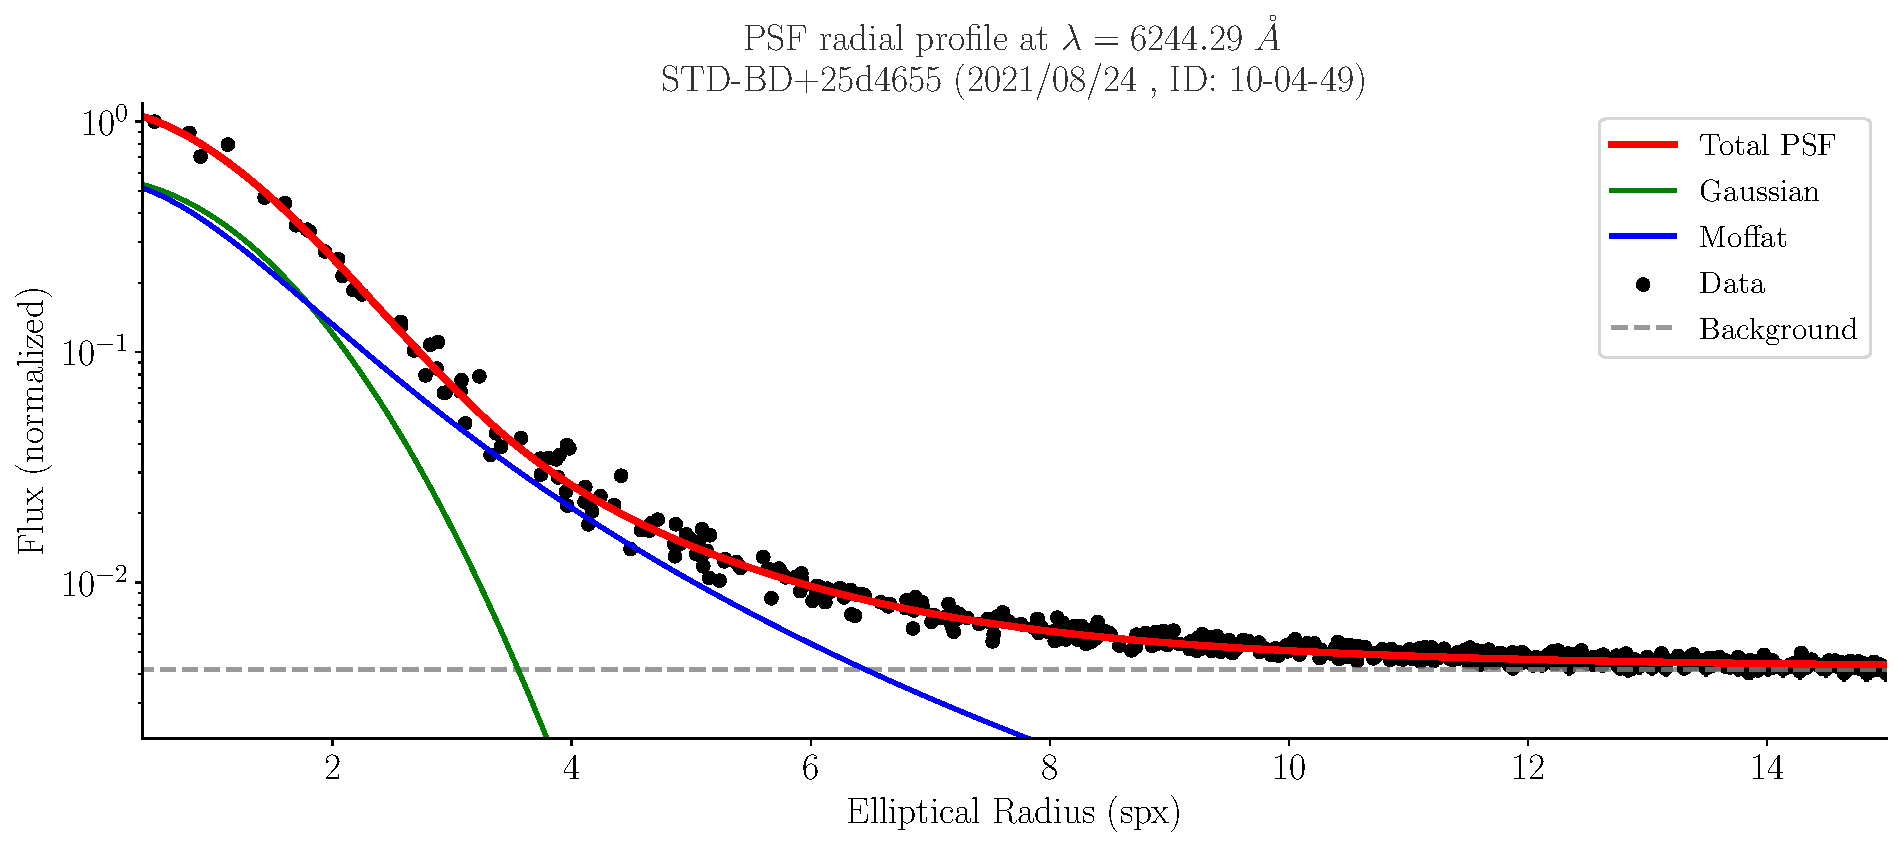
\includegraphics[width=0.99\textwidth]{../figures/06_irf/psfprofile.pdf}
  \caption[Exemple de profil radial d'un étoile standard]{Profil radial
    pour la méta-tranche à $6244$\AA\ de l'étoile standard 25d4655.}
  \label{fig:radialprofile}
\end{figure}

\subsection{Entrainement du modèle}\label{ssec:psftraining}

Notre modèle de PSF contient ainsi $4$ paramètres de forme ($\eta$,
$\alpha$, $\beta$, $\sigma$) et $2$ paramètres de focalisation décrivant
l'ellipticité et l'orientation. Ces $6$ paramètres sont cependant à
priori chromatiques, et le nombre de degré de liberté pour décrire une
simple source ponctuelle devient trop important.

Nous nous sommes ainsi penchés sur l'étude des corrélations entre ces
paramètres et leur chromaticité, afin de contraindre notre modèle de
PSF. Pour faire cela, nous avons utilisé environ $150$ cubes de
données d'étoiles standards, observées avec la SEDm en 2021 toutes saisons
confondues. 

Dans un premier temps, nous procédons à un ajustement avec la fonction
d'étalement de point entièrement libre, pour 9 méta-slices indépendantes
entre $4500$ et $9000$ \AA. Nous avons choisi de ne pas considérer les
longueurs d'ondes au delà de ces extrémités à cause des artefacts trop intenses
générés lors de l'extraction des spectres du CCD, pouvant aller jusqu'à
masquer la source astronomique dans le champ de vue du MLA.

Nous avons ainsi commencé par chercher quels paramètres présentaient la
plus forte corrélation avec les autres. La
Figure~\ref{fig:stdcorrmatrix} met ainsi en évidence, d'une part, une très forte
corrélation entre $\alpha$ et $\beta$, mais également le fait que
$\alpha$ semble montrer le plus de corrélation avec les autres
paramètres de forme. Nous choisissons ainsi $\alpha$ comme paramètre
directeur de notre modèle de PSF.

\begin{figure}[ht]
  \begin{minipage}[c]{0.4\textwidth}
    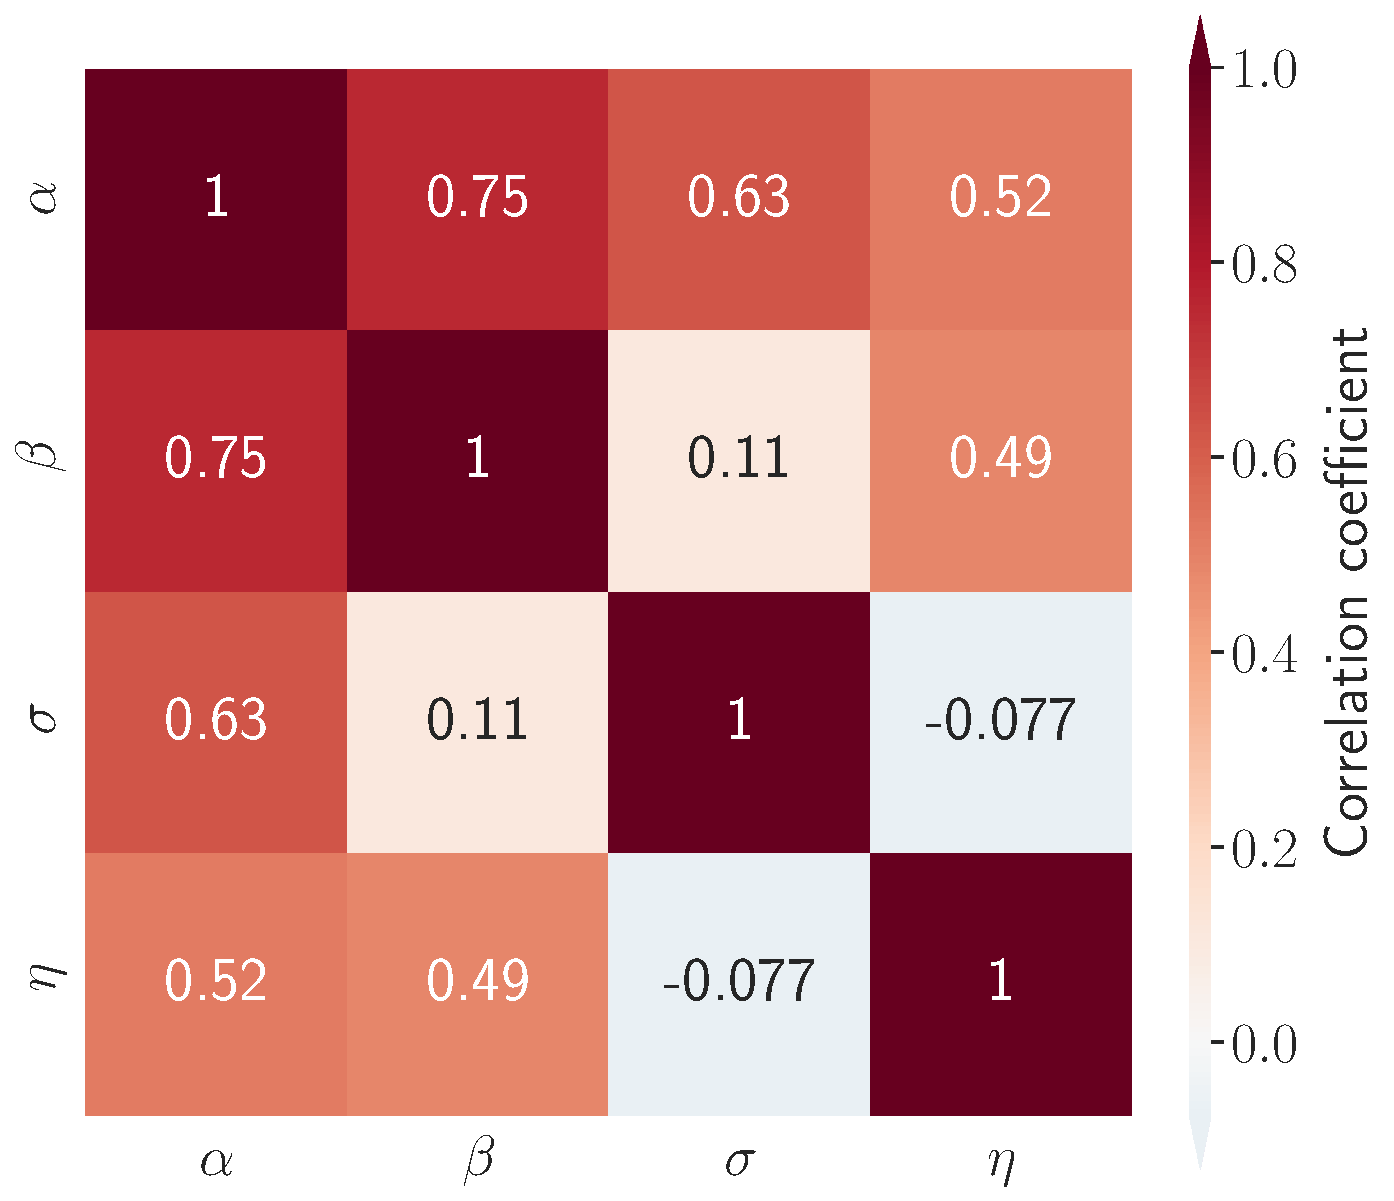
\includegraphics[width=\textwidth]{../figures/06_irf/STD_correlation.pdf}
  \end{minipage}\hfill
  \begin{minipage}[c]{0.53\textwidth}
    \caption[Matrice de corrélation des paramètres de PSF.]{Matrice de
      corrélation des paramètres de PSF toutes méta-tranches confondues,
    avec tous les paramètres libres.}\label{fig:stdcorrmatrix}
  \end{minipage}
\end{figure}

L'idée est alors de fixer adéquatement les corrélations entre les
paramètres, puis de ré-entraîner le modèle de PSF avec ses nouvelles
contraintes. On vérifie alors à nouveau la présence ou non d'autres fortes
corrélations, et nous les fixons successivement.

Cet entrainement est également réalisé chromatiquement. En effet, même
si 2 paramètres sont fortement corrélés sur l'ensemble de l'interval
spectral étudié, nous ne
savons pas a priori si la forme de ces corrélations sont, ou non,
chromatiques. Nous analysons ainsi l'évolution de ces corrélations en
fonction de la longueur d'onde.

\subsubsection{Première contrainte: $\alpha$ vs $\beta$}

Le rayon ($\alpha$) et l'exposant ($\beta$) de la Moffat sont les deux
paramètres qui présentent la plus forte corrélation et de façon significative, nous commençons
donc par fixer celle ci. Nous présentons dans la
Figure~\ref{fig:alphabetachromcorr} les ajustements linéaires pour
chaque méta-tranche. Cet ajustement est effectué par minimisation de
$\chi^{2}$, en pondérant donc par les erreurs.


\begin{figure}[ht]
  \centering
  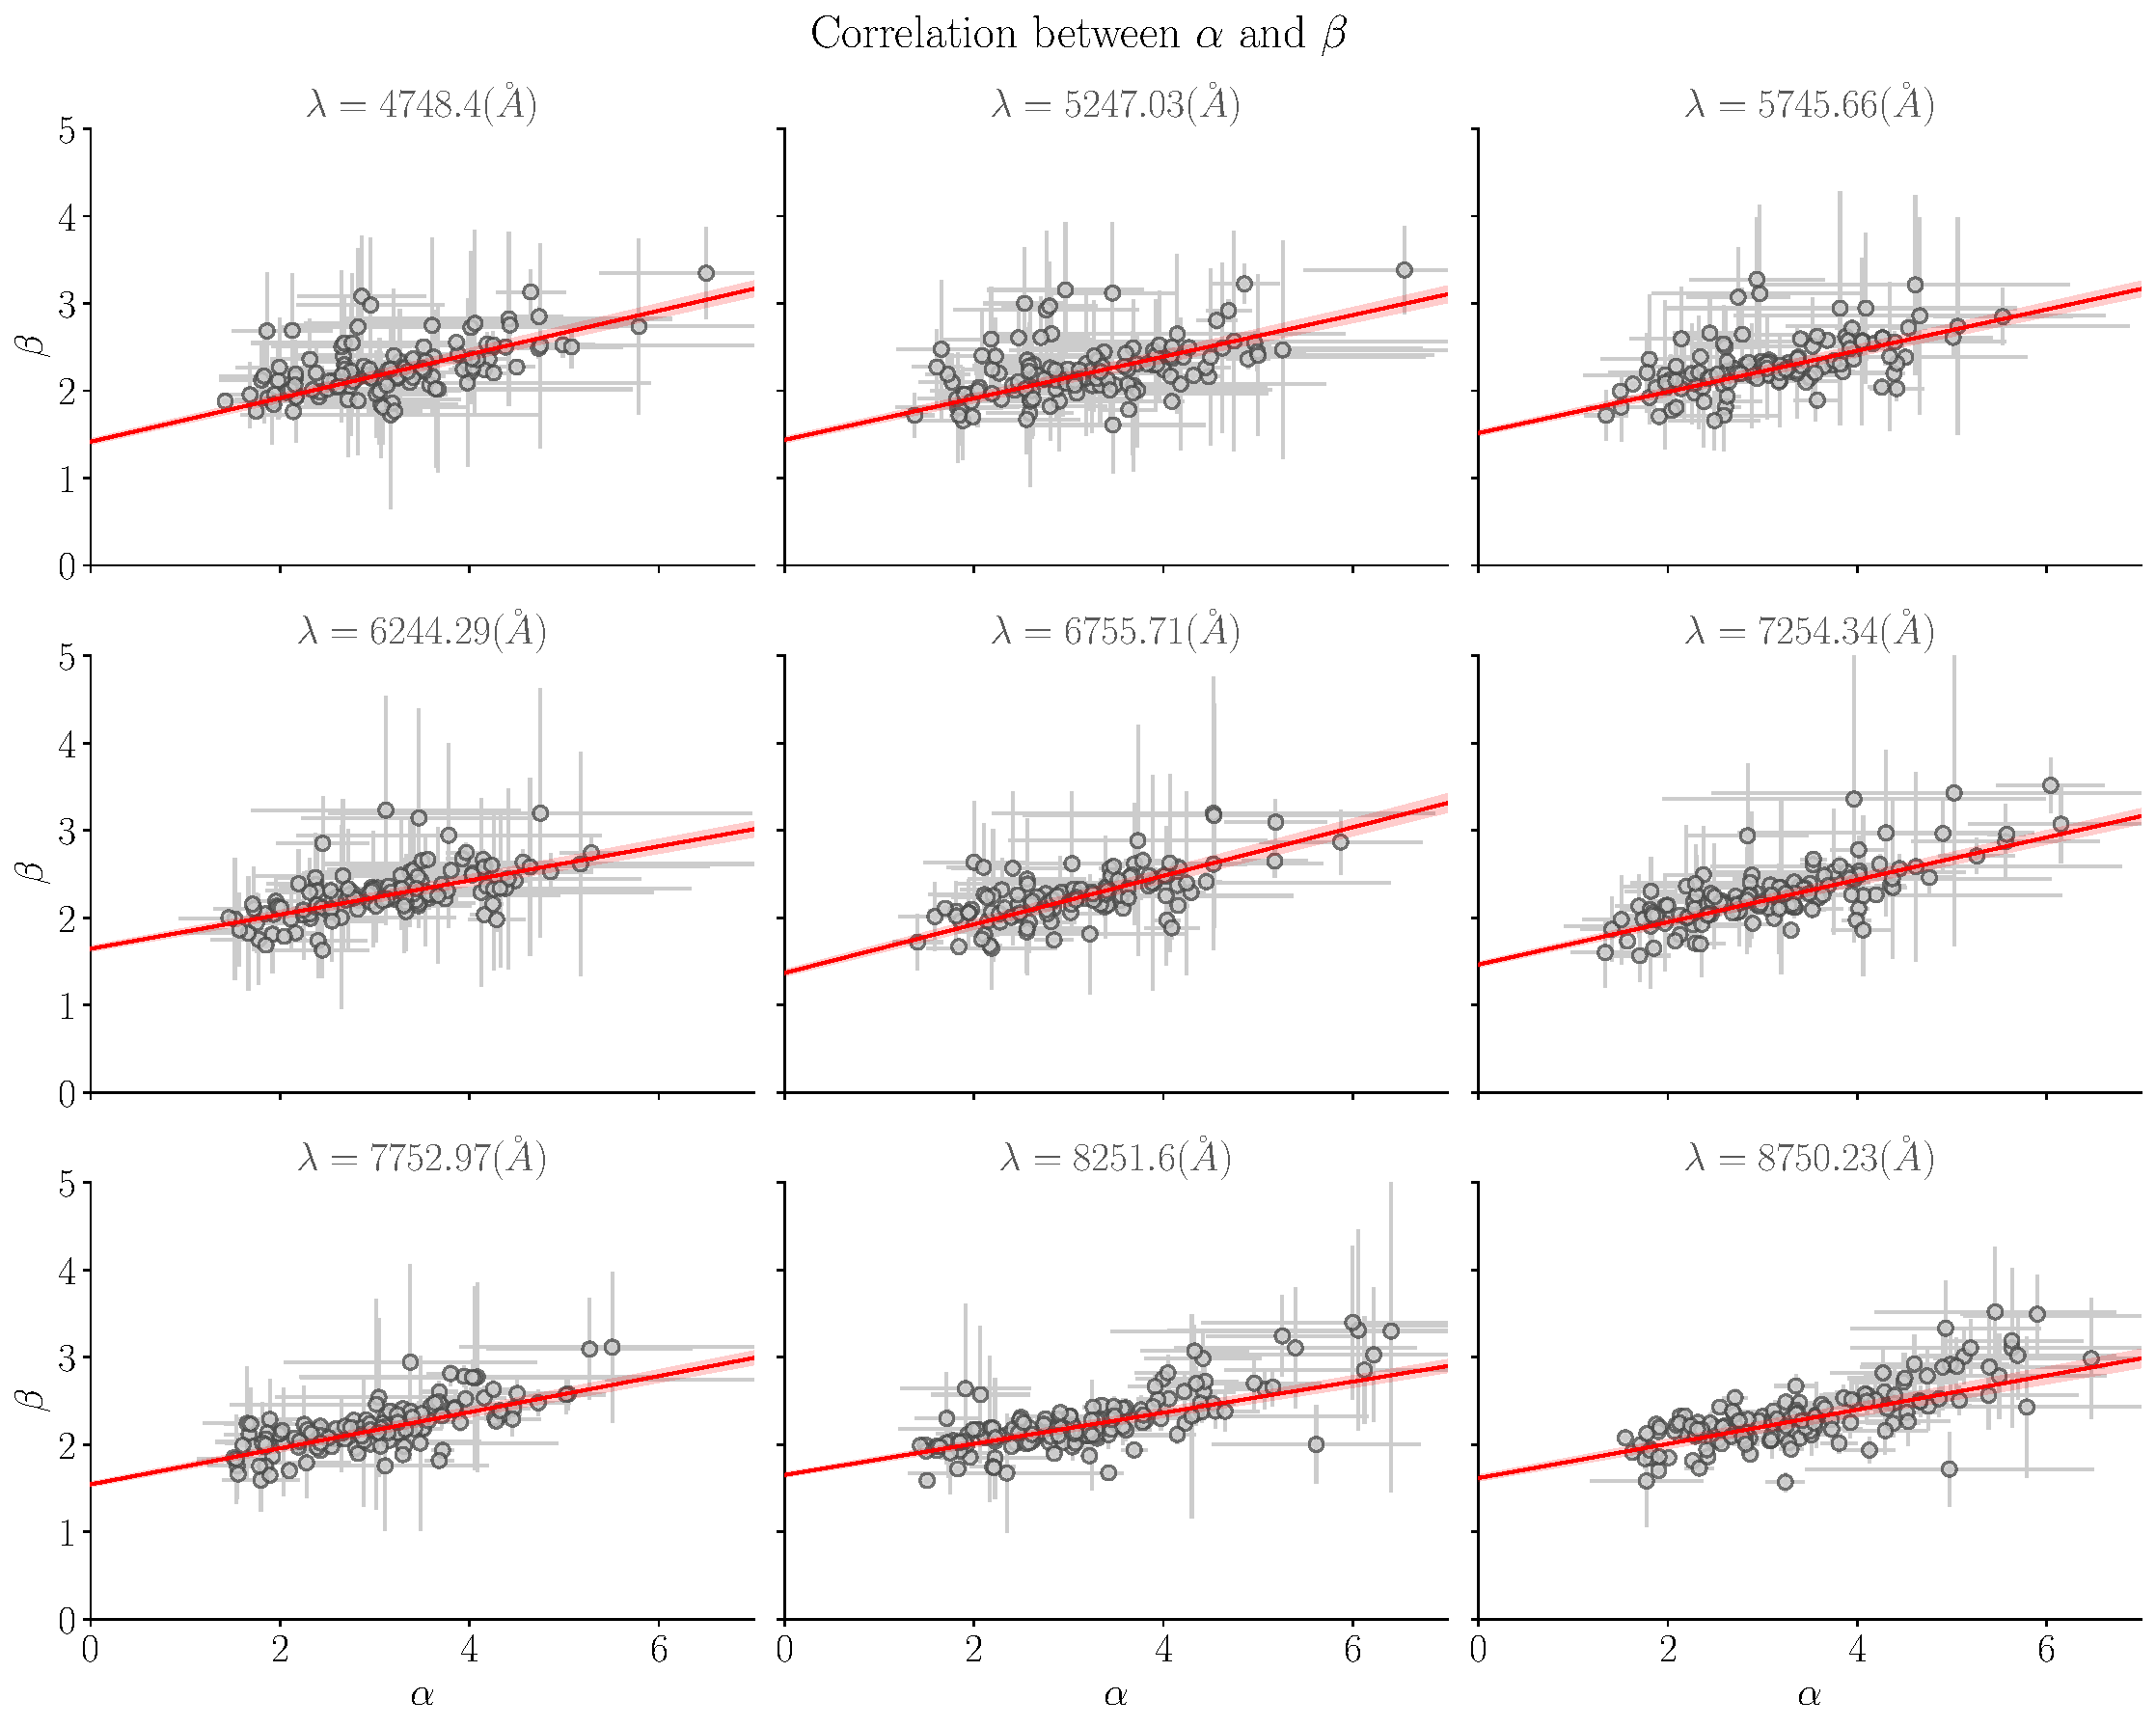
\includegraphics[width=0.8\textwidth]{../figures/06_irf/STD_alpha_beta_chromatic_corr.pdf}
  \caption[Chromaticité des corrélations entre $\alpha$ et $\beta$]{Chromaticité des corrélations entre $\alpha$ et $\beta$}
  \label{fig:alphabetachromcorr}
\end{figure}

La chromaticité de ces ajustements est représenté dans la
Figure~\ref{fig:chromslope_zp_alphabeta}, où nous montrons l'évolution
du point zéro (ordonnée à l'origine) et de la pente en fonction de la
longueur d'onde de la meta-tranche considéré. On observe des effets
chromatiques de l'ordre de $12\%$ pour la pente, et de $6\%$ pour le
point zéro.
Nous avons choisi d'ignorer ces effets chromatiques, et de fixer
$\beta(\alpha)$ indépendamment de la longueur d'onde comme une
combinaison linéaire tel que

\begin{equation}
  \label{eq:betaalpha}
  \beta(\alpha) = \beta_{1}\times \alpha + \beta_{0}
\end{equation}

Avec $\beta_{1}$ et $\beta_{0}$ fixés.

\begin{figure}[ht]
  \centering
  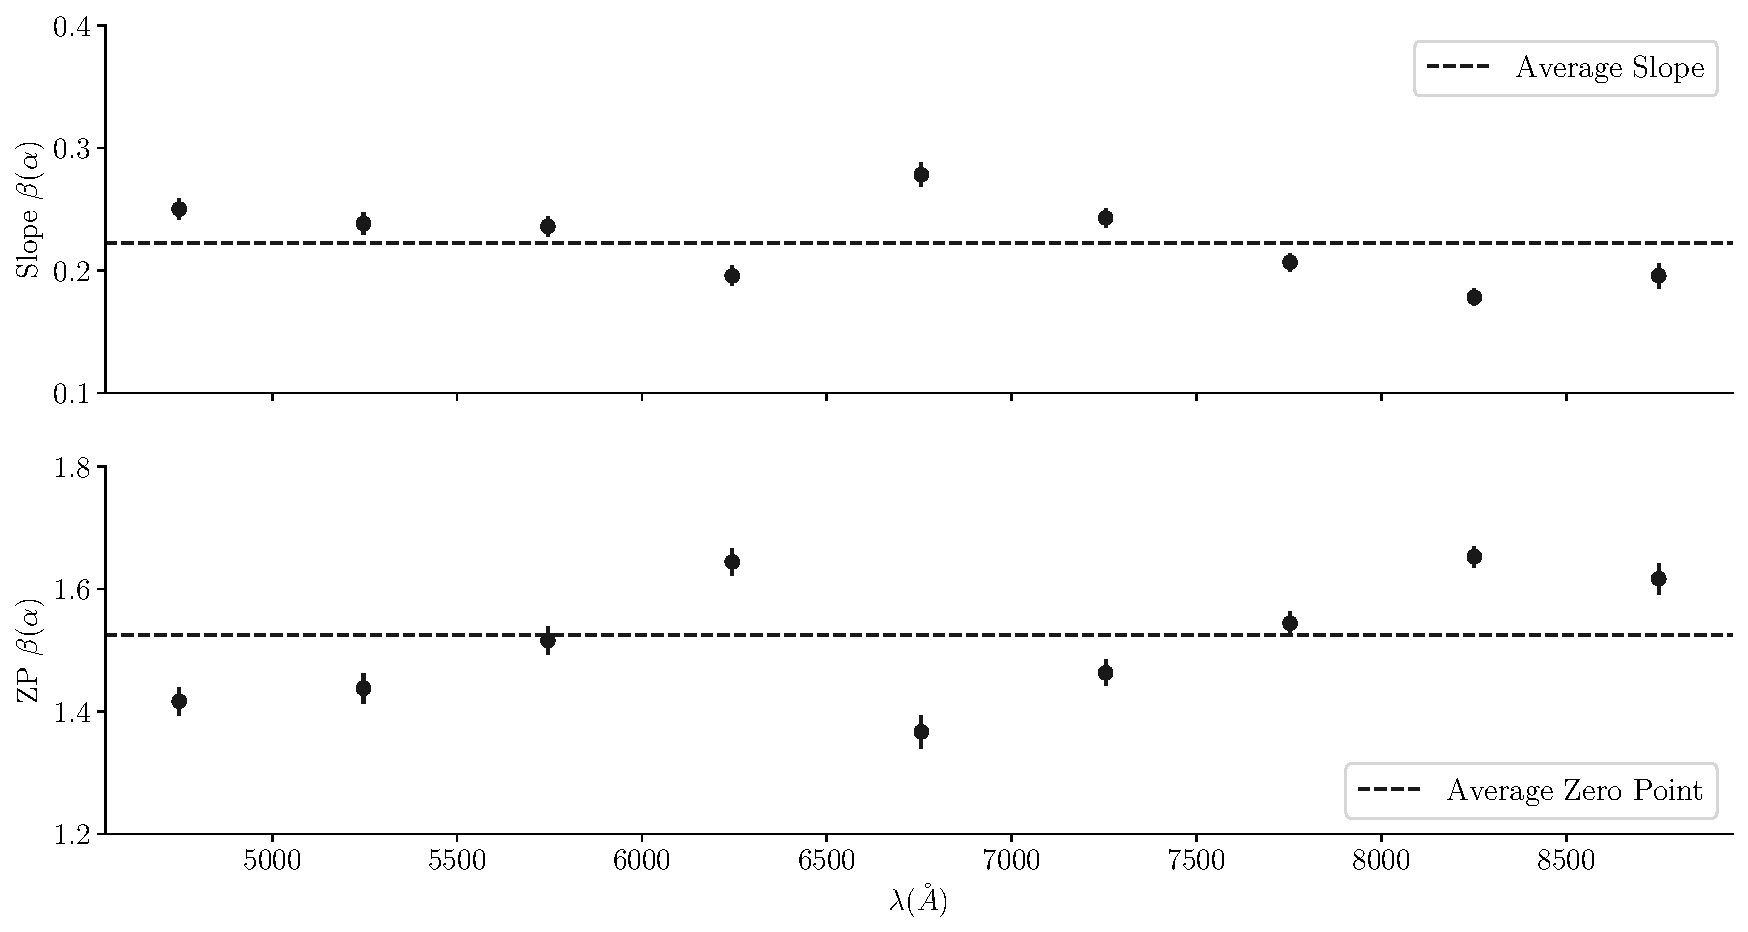
\includegraphics[width=0.7\textwidth]{../figures/06_irf/chromaticitybeta_alpha_corr.pdf}
  \caption[Chromaticité de la pente et du point zéro entre $\alpha$ et $\beta$]{Chromaticité de la pente et du point zéro entre $\alpha$ et $\beta$}
  \label{fig:chromslope_zp_alphabeta}
\end{figure}

%\begin{figure}[ht]
%  \centering
%  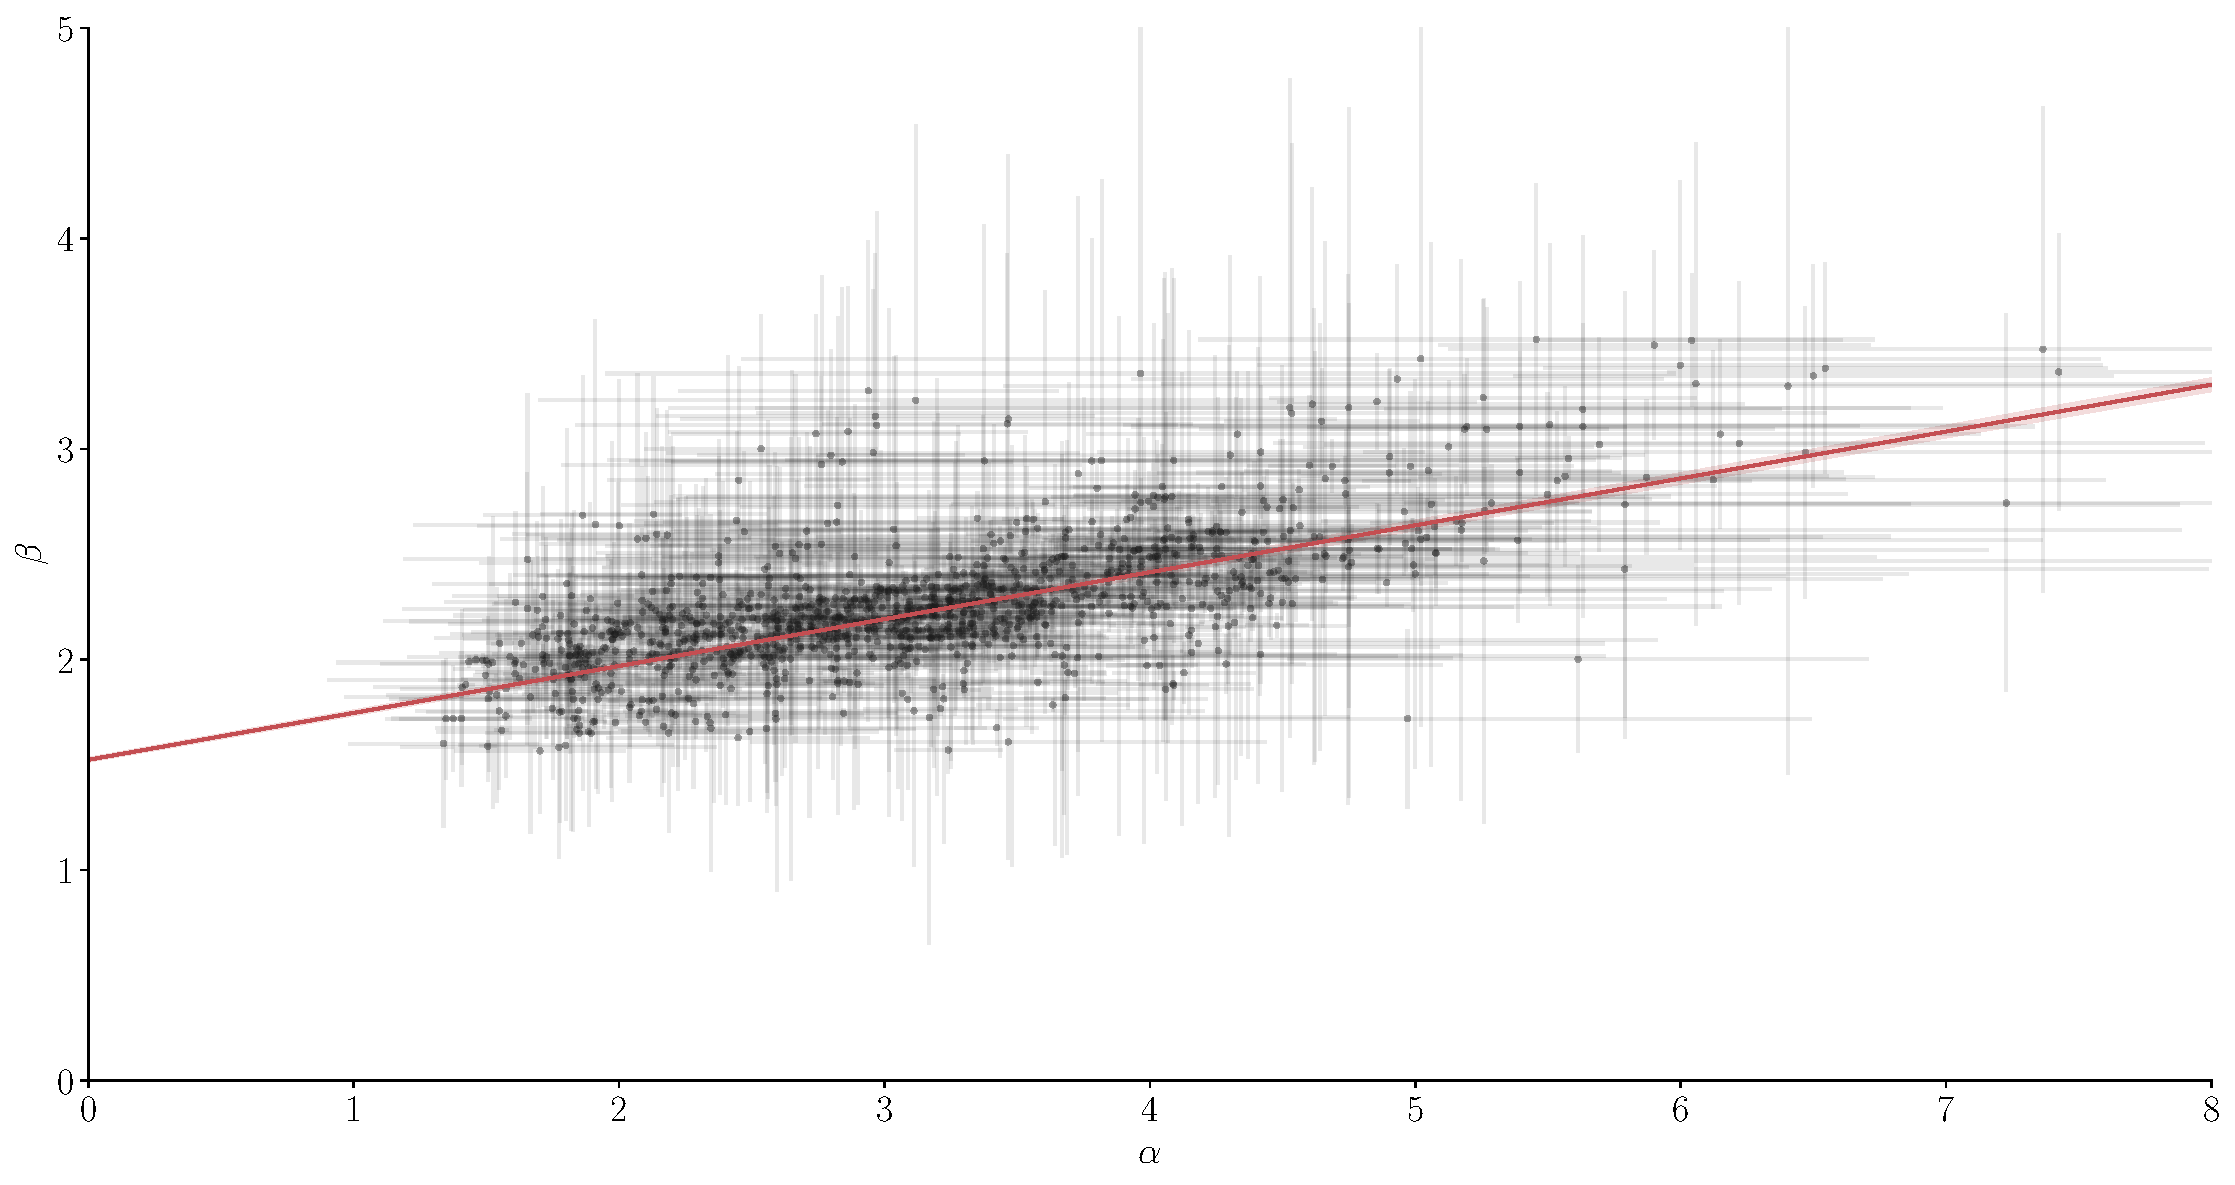
\includegraphics[width=0.8\textwidth]{../figures/06_irf/STD_alpha_beta_corr.pdf}
%  \caption[]{}
%  \label{fig:corralphabeta_achrom}
%\end{figure}

\subsubsection{Seconde contrainte: $\alpha$ vs $\sigma$}


Après avoir fixé la corrélation entre $\alpha$ et $\beta$, on effectue
une nouvelle fois l'ajustement du modèle de PSF pour les mêmes étoiles
standards utilisées précédemment. Nous montrons dans la
Figure~\ref{fig:stdcorrmatrixbetafixed} la nouvelle matrice de
corrélation entre les paramètres de forme en négligeant la chromaticité,
le but étant juste d'avoir une estimation des paramètres présentant les
plus fortes corrélations.


\begin{figure}[ht]
  \begin{minipage}[c]{0.4\textwidth}
    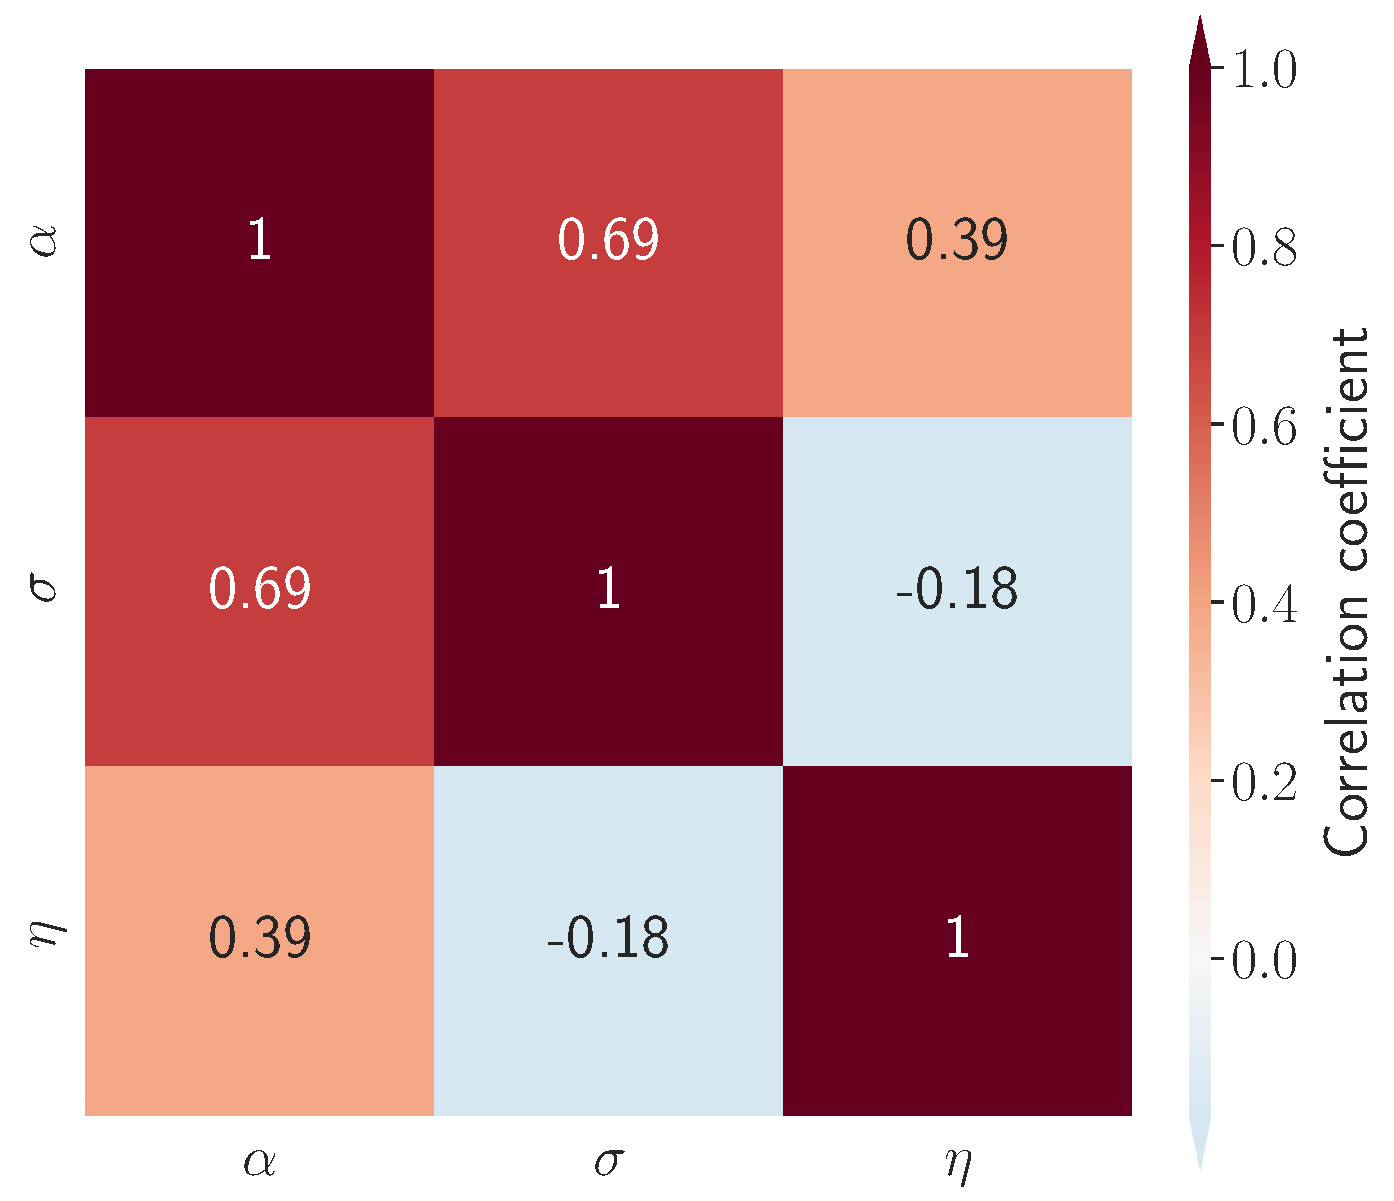
\includegraphics[width=\textwidth]{../figures/06_irf/STD_correlation_matrix_betafixed.pdf}
  \end{minipage}\hfill
  \begin{minipage}[c]{0.53\textwidth}
    \caption[Matrice de corrélation des paramètres de PSF ($\beta(\alpha)$ fixé).]{Matrice de
      corrélation des paramètres de PSF toutes méta-tranches confondues,
    après fixation de $\beta(\alpha)$.}\label{fig:stdcorrmatrixbetafixed}
  \end{minipage}
\end{figure}

Nous nous intéressons donc à présent à la relation entre $\alpha$ (le
rayon de la Moffat) et $\sigma$, le rayon de la gaussienne.

De la même manière que précédemment, nous présentons dans la
Figure~\ref{fig:alphasigmachromcorr} les ajustements linéaires entre ces
deux paramètres pour chaque méta-tranche. Il est à noter que cette
corrélation est presque aussi significative que celle entre $\alpha$ et
$\beta$, ce qui montre à quel point ces trois paramètres sont corrélés
entre eux.


\begin{figure}[ht]
  \centering
  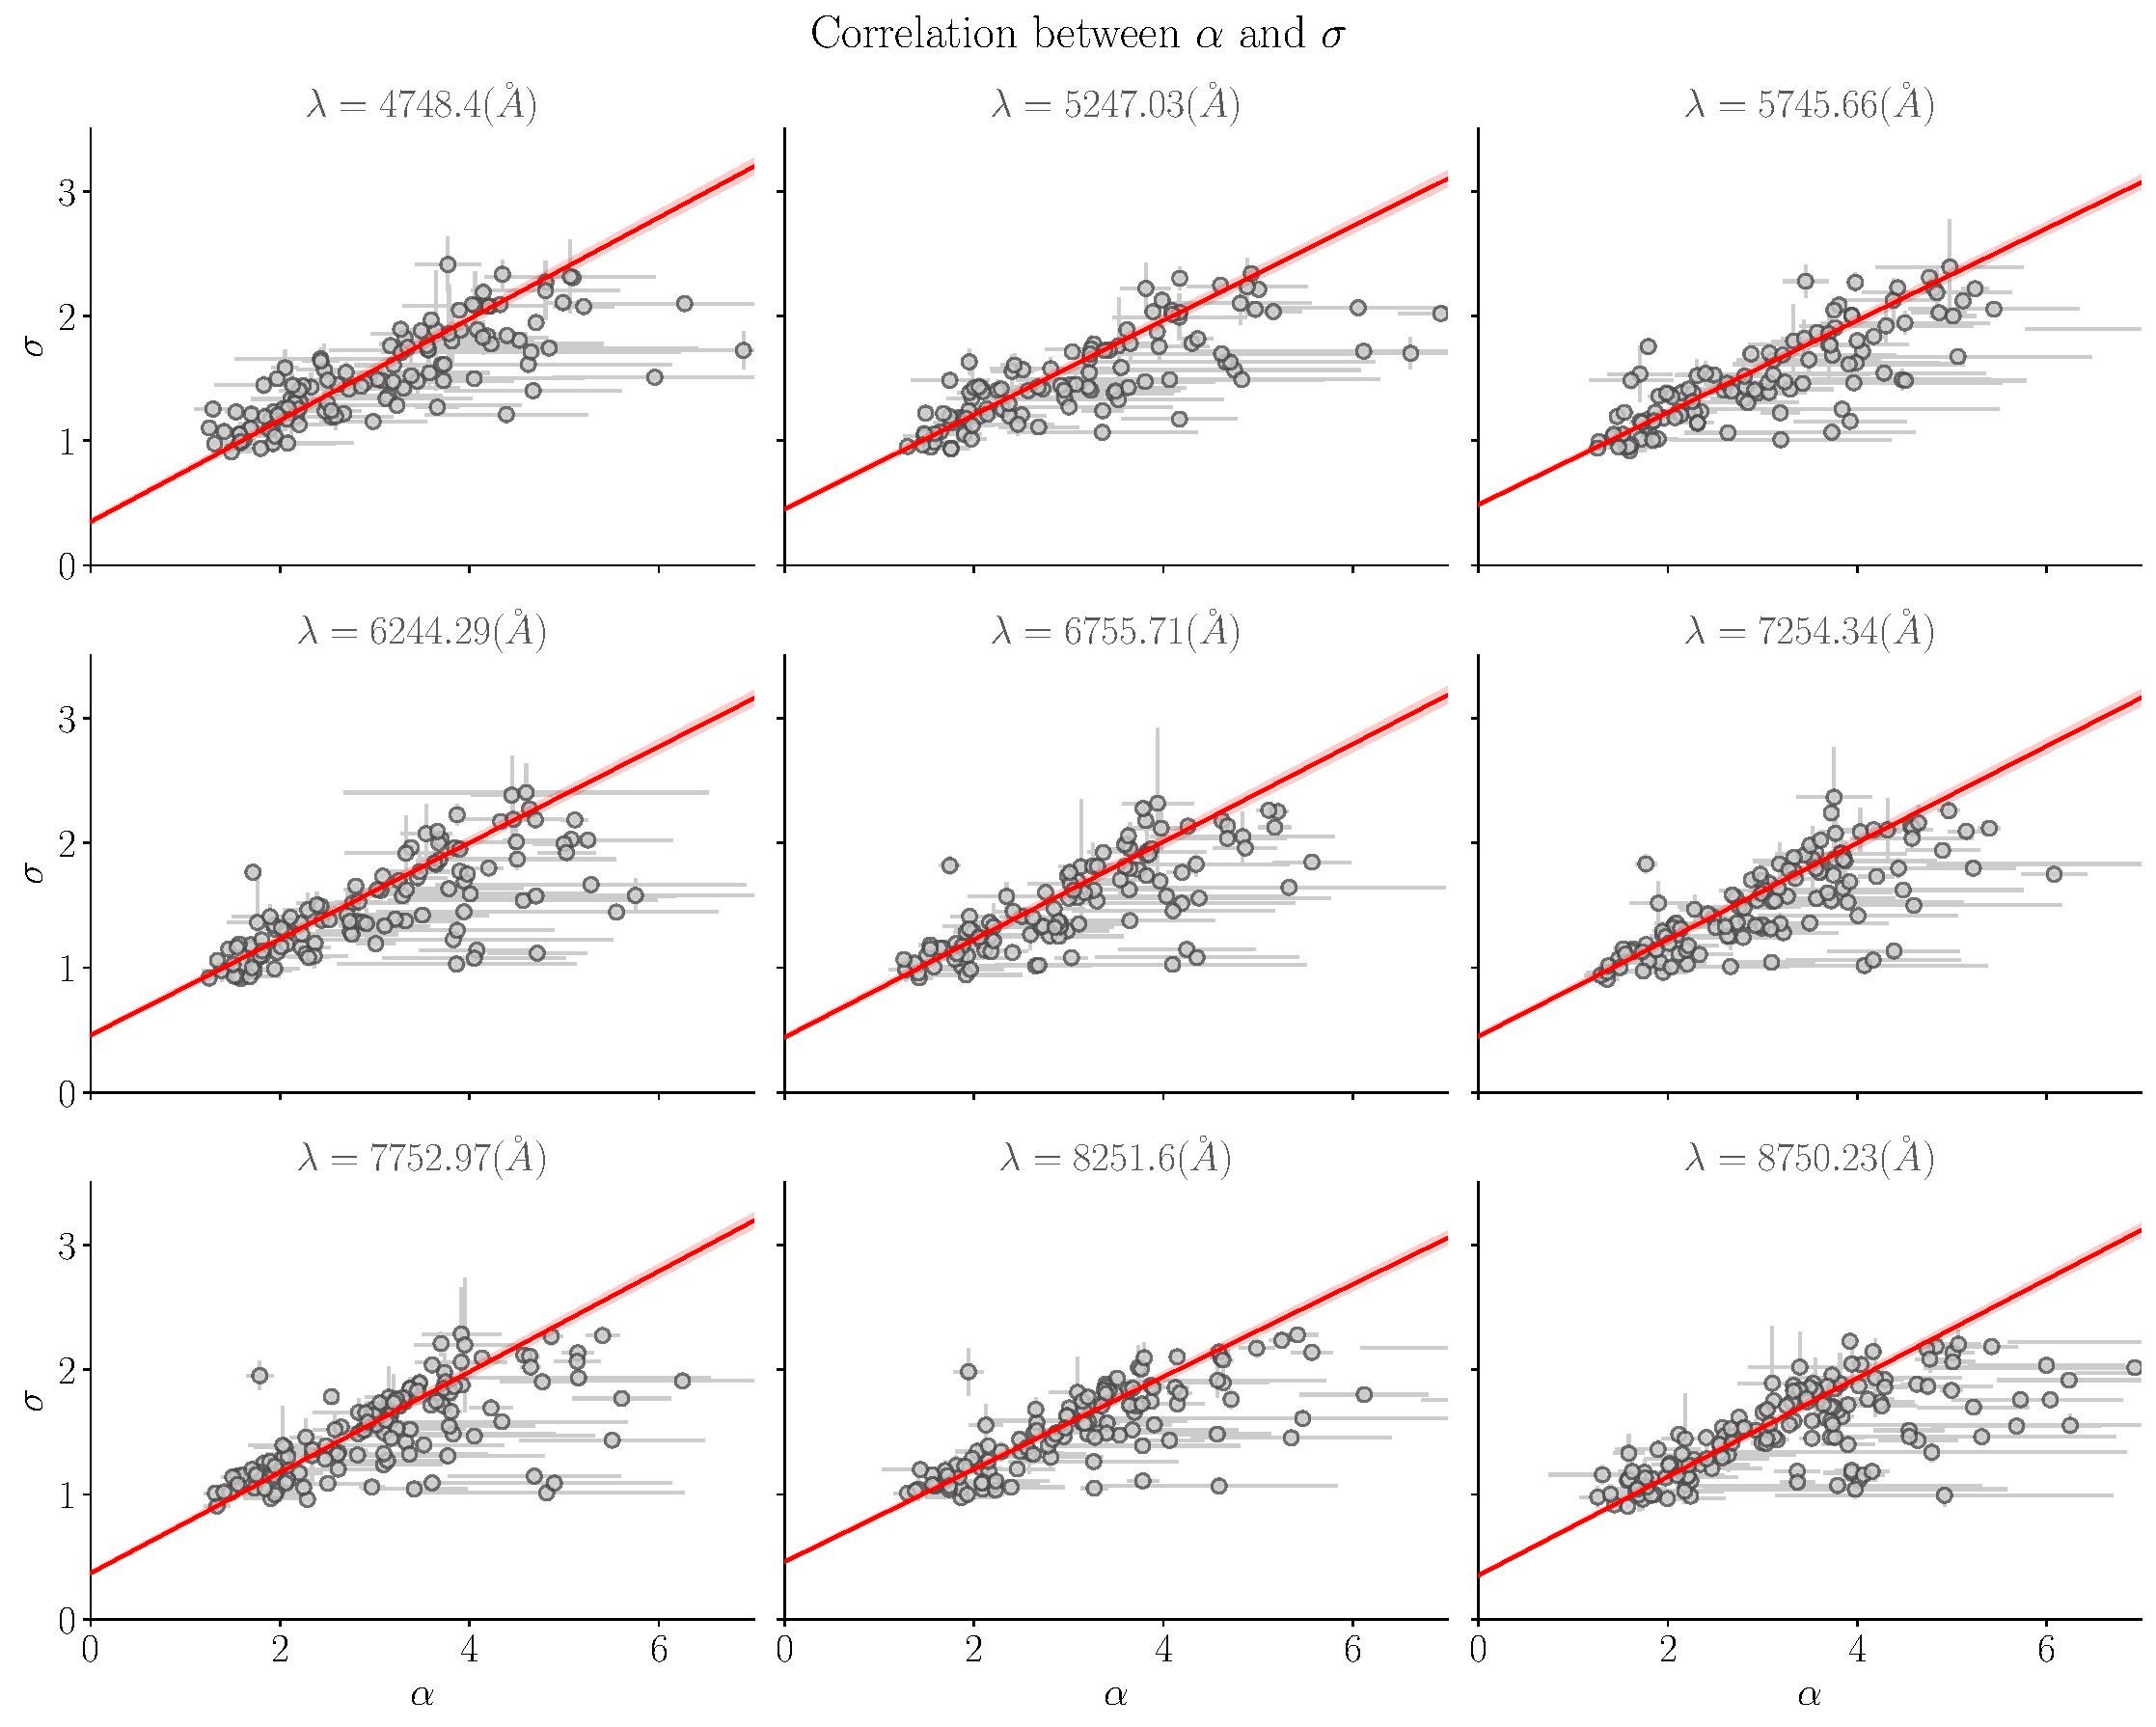
\includegraphics[width=0.8\textwidth]{../figures/06_irf/STD_alpha_sigma_chromatic_corr.pdf}
  \caption[Chromaticité des corrélations entre $\alpha$ et $\sigma$]{Chromaticité des corrélations entre $\alpha$ et $\sigma$}
  \label{fig:alphasigmachromcorr}
\end{figure}

Tout comme précédement, la chromaticité de ces ajustements est représenté dans la
Figure~\ref{fig:chromslope_zp_alphasigma}, où nous montrons l'évolution
du point zéro et de la pente en fonction de la
longueur d'onde de la meta-tranche considéré. On observe cette fois ci des effets
chromatiques de l'ordre de seulement $3\%$ pour la pente, et de $8\%$ pour le
point zéro.
Nous avons à nouveau choisi d'ignorer ces effets chromatiques, et de fixer
$\sigma(\alpha)$ indépendamment de la longueur d'onde comme une
combinaison linéaire tel que

\begin{equation}
  \label{eq:betaalpha}
  \sigma(\alpha) = \sigma_{1}\times \alpha + \sigma_{0}
\end{equation}

Avec $\sigma_{1}$ et $\sigma_{0}$ fixés.

\begin{figure}[ht]
  \centering
  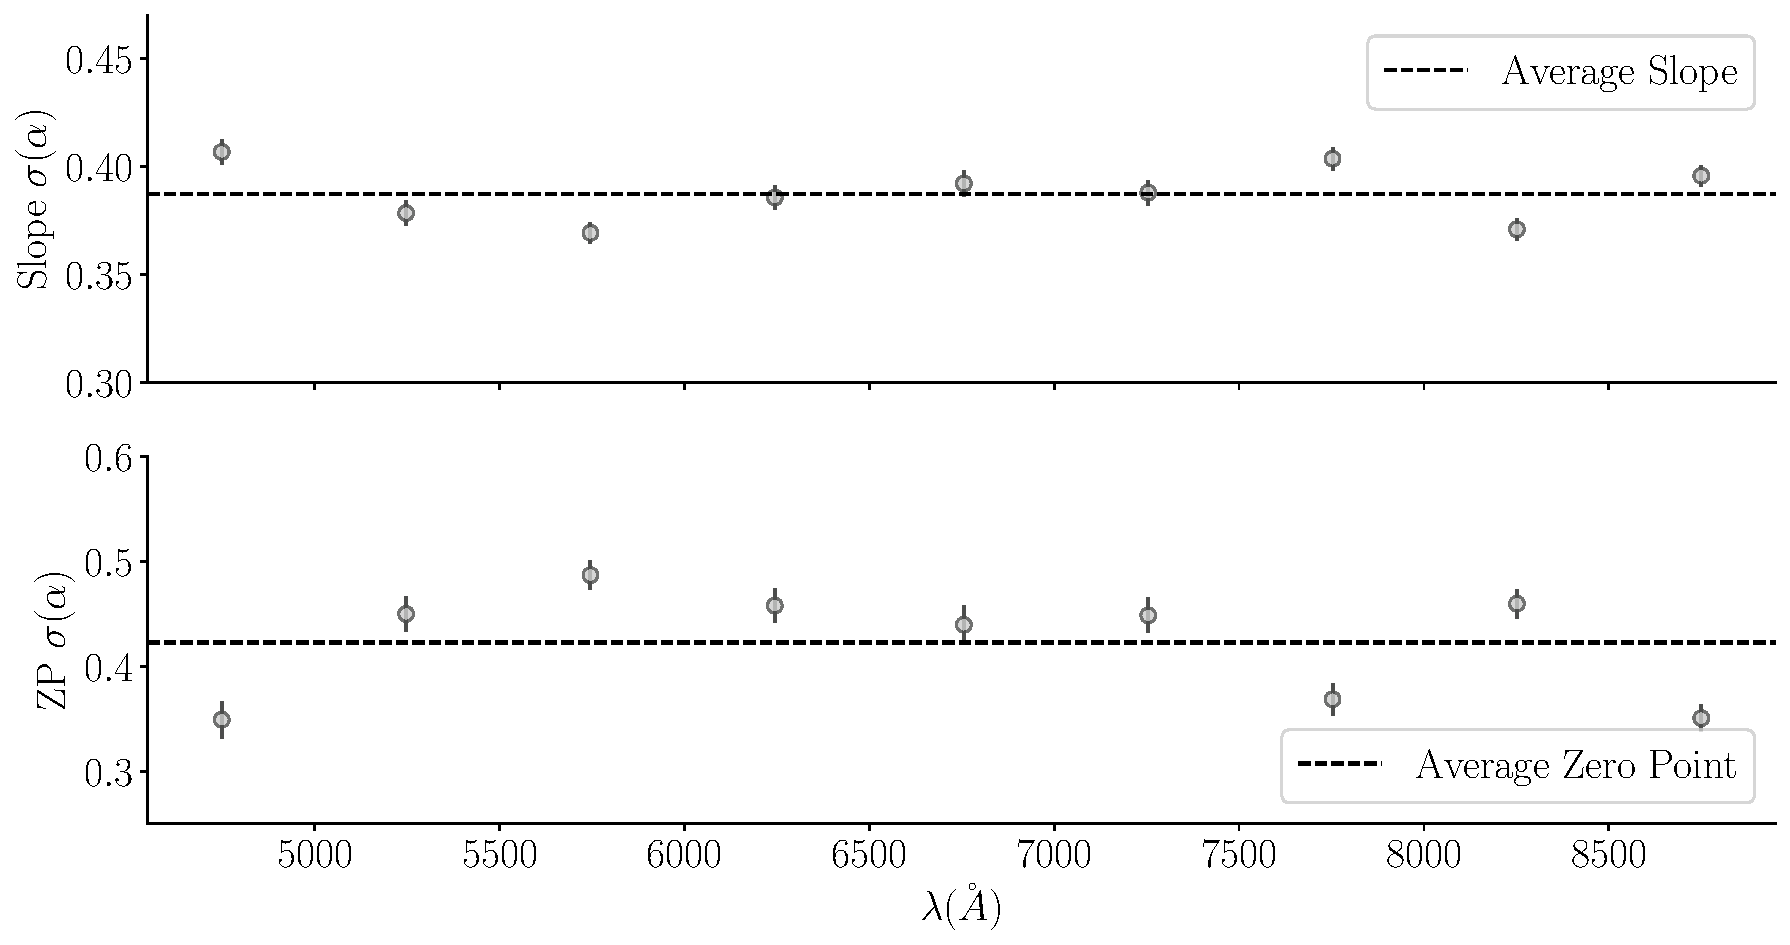
\includegraphics[width=0.7\textwidth]{../figures/06_irf/chromaticitysigma_alpha_corr.pdf}
  \caption[Chromaticité de la pente et du point zéro entre $\alpha$ et $\sigma$]{Chromaticité de la pente et du point zéro entre $\alpha$ et $\sigma$}
  \label{fig:chromslope_zp_alphasigma}
\end{figure}

%\begin{figure}[ht]
%  \centering
%  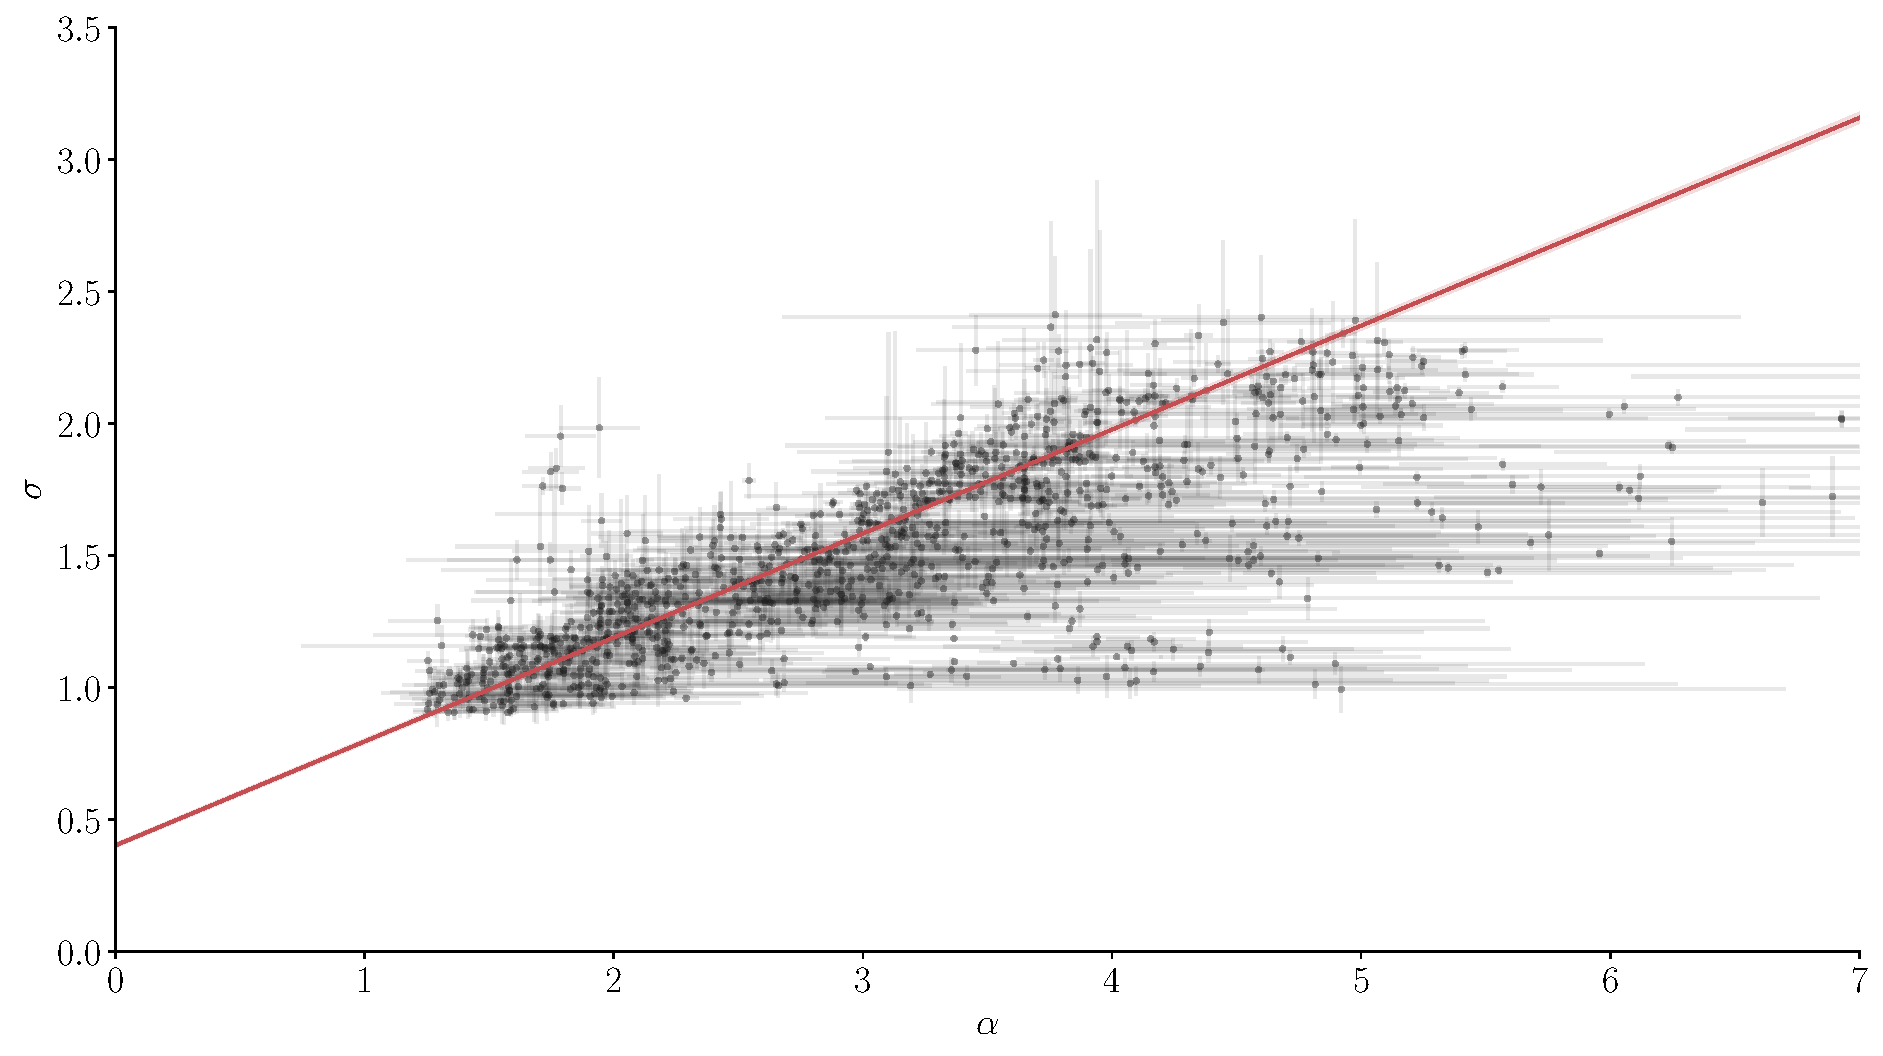
\includegraphics[width=0.8\textwidth]{../figures/06_irf/STD_correlation_betafixed.pdf}
%  \caption[]{}
%  \label{fig:corralphasigma_achrom}
%\end{figure}


\begin{figure}[ht]
  \centering
  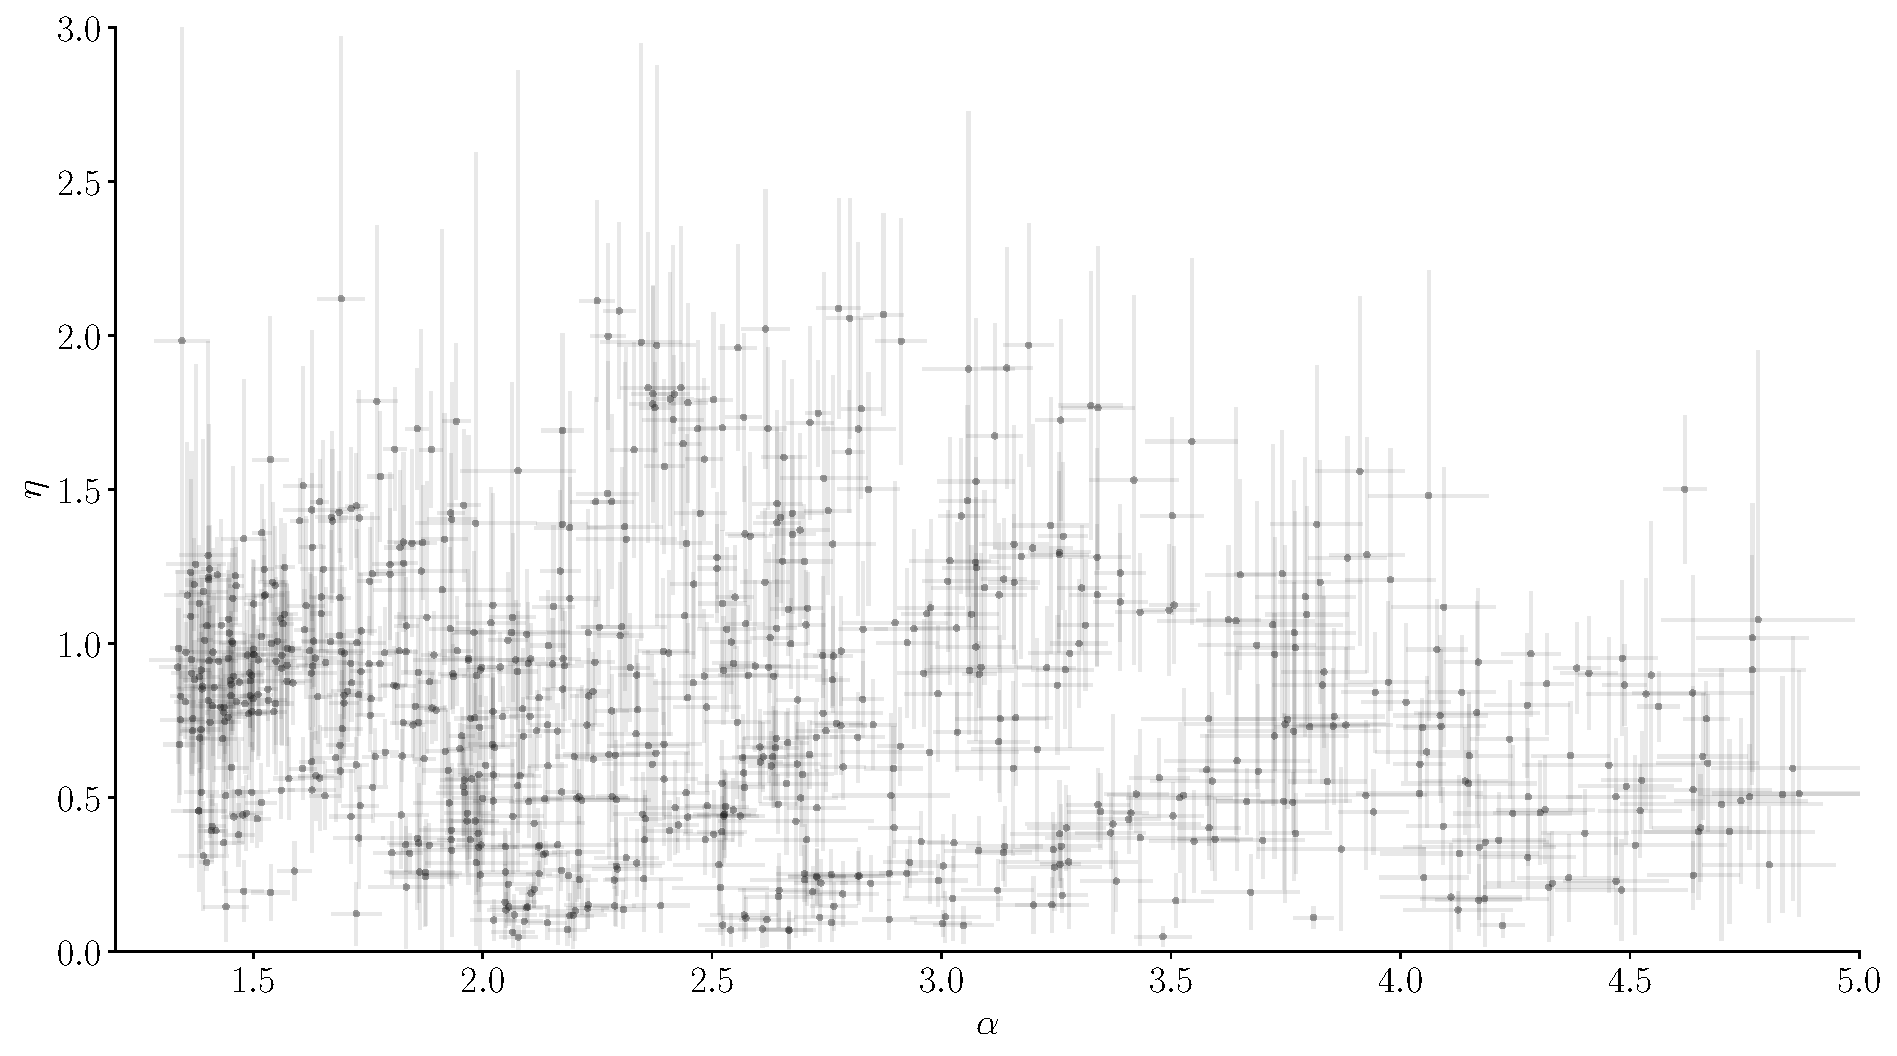
\includegraphics[width=0.8\textwidth]{../figures/06_irf/STD_correlation_betasigmafixed.pdf}
  \caption[]{}
  \label{fig:}
\end{figure}



\begin{figure}[ht]
  \centering
  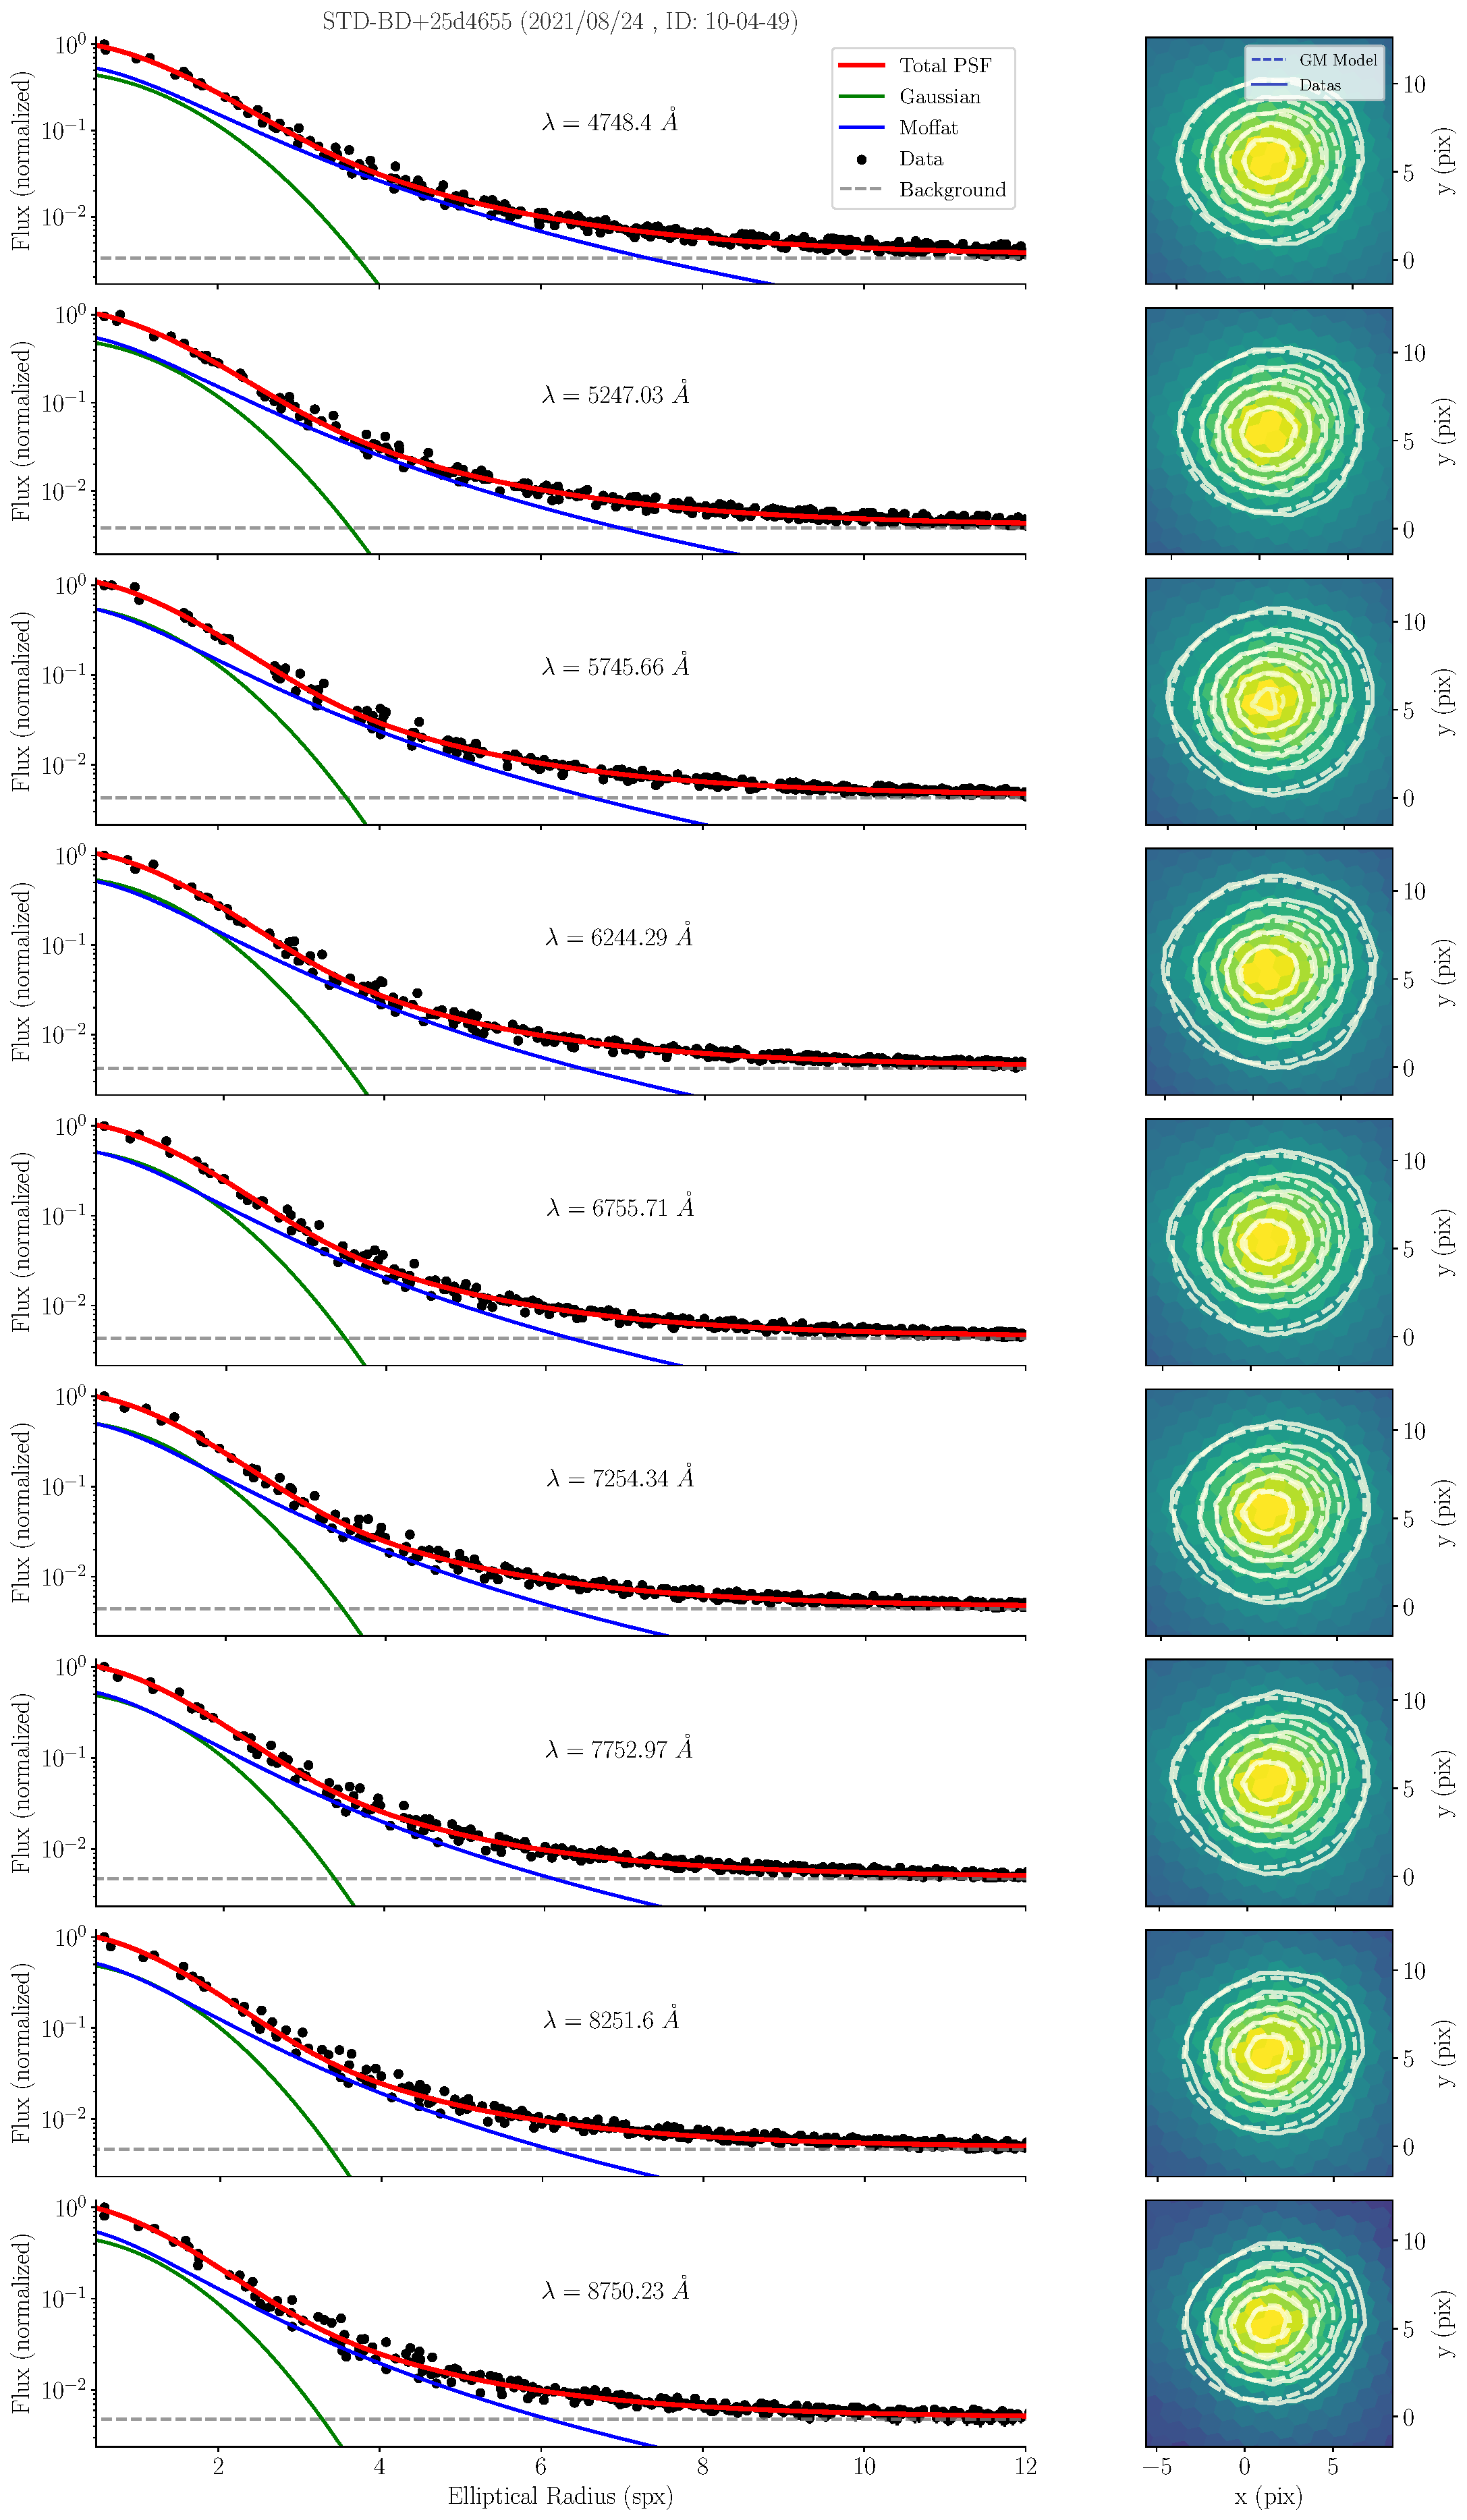
\includegraphics[width=0.7\textwidth]{../figures/06_irf/STD_profile_allmeta.pdf}
  \caption[]{Profil radial et coutours des $9$ metaslices de la STD}
  \label{fig:}
\end{figure}

\subsection{Chromaticité et ADR}\label{ssec:chromadr}

\section{Validation}\label{sec:validationpsf}

\subsection{Calibration photométrique}\label{ssec:photocalibstd}

\subsection{Résultats}\label{ssec:resultscalib}


\bibliographystyle{../main/aa_url2}
\bibliography{99_references}

\end{document}

%%% Local Variables:
%%% mode: latex
%%% TeX-master: t
%%% End:
